\documentclass[ignorenonframetext,]{beamer}
\setbeamertemplate{caption}[numbered]
\setbeamertemplate{caption label separator}{: }
\setbeamercolor{caption name}{fg=normal text.fg}
\beamertemplatenavigationsymbolsempty
\usepackage{lmodern}
\usepackage{amssymb,amsmath}
\usepackage{ifxetex,ifluatex}
\usepackage{fixltx2e} % provides \textsubscript
\ifnum 0\ifxetex 1\fi\ifluatex 1\fi=0 % if pdftex
  \usepackage[T1]{fontenc}
  \usepackage[utf8]{inputenc}
\else % if luatex or xelatex
  \ifxetex
    \usepackage{mathspec}
  \else
    \usepackage{fontspec}
  \fi
  \defaultfontfeatures{Ligatures=TeX,Scale=MatchLowercase}
\fi
% use upquote if available, for straight quotes in verbatim environments
\IfFileExists{upquote.sty}{\usepackage{upquote}}{}
% use microtype if available
\IfFileExists{microtype.sty}{%
\usepackage{microtype}
\UseMicrotypeSet[protrusion]{basicmath} % disable protrusion for tt fonts
}{}
\newif\ifbibliography
\hypersetup{
            pdftitle={Module 3: LINEAR REGRESSION},
            pdfauthor={Mette Langaas, Department of Mathematical Sciences, NTNU},
            pdfborder={0 0 0},
            breaklinks=true}
\urlstyle{same}  % don't use monospace font for urls
\usepackage{color}
\usepackage{fancyvrb}
\newcommand{\VerbBar}{|}
\newcommand{\VERB}{\Verb[commandchars=\\\{\}]}
\DefineVerbatimEnvironment{Highlighting}{Verbatim}{commandchars=\\\{\}}
% Add ',fontsize=\small' for more characters per line
\usepackage{framed}
\definecolor{shadecolor}{RGB}{248,248,248}
\newenvironment{Shaded}{\begin{snugshade}}{\end{snugshade}}
\newcommand{\KeywordTok}[1]{\textcolor[rgb]{0.13,0.29,0.53}{\textbf{#1}}}
\newcommand{\DataTypeTok}[1]{\textcolor[rgb]{0.13,0.29,0.53}{#1}}
\newcommand{\DecValTok}[1]{\textcolor[rgb]{0.00,0.00,0.81}{#1}}
\newcommand{\BaseNTok}[1]{\textcolor[rgb]{0.00,0.00,0.81}{#1}}
\newcommand{\FloatTok}[1]{\textcolor[rgb]{0.00,0.00,0.81}{#1}}
\newcommand{\ConstantTok}[1]{\textcolor[rgb]{0.00,0.00,0.00}{#1}}
\newcommand{\CharTok}[1]{\textcolor[rgb]{0.31,0.60,0.02}{#1}}
\newcommand{\SpecialCharTok}[1]{\textcolor[rgb]{0.00,0.00,0.00}{#1}}
\newcommand{\StringTok}[1]{\textcolor[rgb]{0.31,0.60,0.02}{#1}}
\newcommand{\VerbatimStringTok}[1]{\textcolor[rgb]{0.31,0.60,0.02}{#1}}
\newcommand{\SpecialStringTok}[1]{\textcolor[rgb]{0.31,0.60,0.02}{#1}}
\newcommand{\ImportTok}[1]{#1}
\newcommand{\CommentTok}[1]{\textcolor[rgb]{0.56,0.35,0.01}{\textit{#1}}}
\newcommand{\DocumentationTok}[1]{\textcolor[rgb]{0.56,0.35,0.01}{\textbf{\textit{#1}}}}
\newcommand{\AnnotationTok}[1]{\textcolor[rgb]{0.56,0.35,0.01}{\textbf{\textit{#1}}}}
\newcommand{\CommentVarTok}[1]{\textcolor[rgb]{0.56,0.35,0.01}{\textbf{\textit{#1}}}}
\newcommand{\OtherTok}[1]{\textcolor[rgb]{0.56,0.35,0.01}{#1}}
\newcommand{\FunctionTok}[1]{\textcolor[rgb]{0.00,0.00,0.00}{#1}}
\newcommand{\VariableTok}[1]{\textcolor[rgb]{0.00,0.00,0.00}{#1}}
\newcommand{\ControlFlowTok}[1]{\textcolor[rgb]{0.13,0.29,0.53}{\textbf{#1}}}
\newcommand{\OperatorTok}[1]{\textcolor[rgb]{0.81,0.36,0.00}{\textbf{#1}}}
\newcommand{\BuiltInTok}[1]{#1}
\newcommand{\ExtensionTok}[1]{#1}
\newcommand{\PreprocessorTok}[1]{\textcolor[rgb]{0.56,0.35,0.01}{\textit{#1}}}
\newcommand{\AttributeTok}[1]{\textcolor[rgb]{0.77,0.63,0.00}{#1}}
\newcommand{\RegionMarkerTok}[1]{#1}
\newcommand{\InformationTok}[1]{\textcolor[rgb]{0.56,0.35,0.01}{\textbf{\textit{#1}}}}
\newcommand{\WarningTok}[1]{\textcolor[rgb]{0.56,0.35,0.01}{\textbf{\textit{#1}}}}
\newcommand{\AlertTok}[1]{\textcolor[rgb]{0.94,0.16,0.16}{#1}}
\newcommand{\ErrorTok}[1]{\textcolor[rgb]{0.64,0.00,0.00}{\textbf{#1}}}
\newcommand{\NormalTok}[1]{#1}
\usepackage{graphicx,grffile}
\makeatletter
\def\maxwidth{\ifdim\Gin@nat@width>\linewidth\linewidth\else\Gin@nat@width\fi}
\def\maxheight{\ifdim\Gin@nat@height>\textheight0.8\textheight\else\Gin@nat@height\fi}
\makeatother
% Scale images if necessary, so that they will not overflow the page
% margins by default, and it is still possible to overwrite the defaults
% using explicit options in \includegraphics[width, height, ...]{}
\setkeys{Gin}{width=\maxwidth,height=\maxheight,keepaspectratio}

% Prevent slide breaks in the middle of a paragraph:
\widowpenalties 1 10000
\raggedbottom

\AtBeginPart{
  \let\insertpartnumber\relax
  \let\partname\relax
  \frame{\partpage}
}
\AtBeginSection{
  \ifbibliography
  \else
    \let\insertsectionnumber\relax
    \let\sectionname\relax
    \frame{\sectionpage}
  \fi
}
\AtBeginSubsection{
  \let\insertsubsectionnumber\relax
  \let\subsectionname\relax
  \frame{\subsectionpage}
}

\setlength{\parindent}{0pt}
\setlength{\parskip}{6pt plus 2pt minus 1pt}
\setlength{\emergencystretch}{3em}  % prevent overfull lines
\providecommand{\tightlist}{%
  \setlength{\itemsep}{0pt}\setlength{\parskip}{0pt}}
\setcounter{secnumdepth}{0}

\title{Module 3: LINEAR REGRESSION}
\subtitle{TMA4268 Statistical Learning V2019}
\author{Mette Langaas, Department of Mathematical Sciences, NTNU}
\date{week 4 2019}

\begin{document}
\frame{\titlepage}

\begin{frame}

Last changes: (18.01: typos corrected)

\end{frame}

\begin{frame}{Introduction}

\begin{block}{Learning material for this module}

\begin{itemize}
\tightlist
\item
  James et al (2013): An Introduction to Statistical Learning. Chapter
  3.
\end{itemize}

We need more statistical theory than is presented in the textbook, which
you find in this module page.

\end{block}

\end{frame}

\begin{frame}

\begin{block}{Topics in this module}

\begin{block}{Part A: Simple linear regression and introduction to
multiple linear regression}

\begin{itemize}
\tightlist
\item
  Aim of linear regression
\item
  Simple linear regression

  \begin{itemize}
  \tightlist
  \item
    model
  \item
    parameter estimation
  \item
    confidence intervals
  \item
    single hypothesis testing: set-up and \(p\)-values
  \item
    model fit
  \end{itemize}
\item
  Multiple linear regression

  \begin{itemize}
  \tightlist
  \item
    model
  \item
    parameter estimation with least squares
  \item
    properties of parameter estimators
  \end{itemize}
\end{itemize}

\end{block}

\end{block}

\end{frame}

\begin{frame}

\begin{block}{Part B: Multiple linear regression - continued}

\begin{itemize}
\tightlist
\item
  So far: simple linear regression - and multiple linear regression -
  model, estimators
\item
  Statistical inference

  \begin{itemize}
  \tightlist
  \item
    estimators and properties
  \item
    confidence intervals and hypothesis tests
  \item
    significance of regression: F-test
  \item
    prediction and prediction intervals
  \end{itemize}
\item
  Model assessement and selection

  \begin{itemize}
  \tightlist
  \item
    \(R^2\)
  \item
    subset selection
  \item
    diagnostic plots - studentized residuals and leverages
  \end{itemize}
\end{itemize}

\end{block}

\end{frame}

\begin{frame}

\begin{itemize}
\tightlist
\item
  Extensions and challenges (self study)

  \begin{itemize}
  \tightlist
  \item
    qualitative predictors: dummy coding (needed)
  \item
    non-additivity: including interactions (useful)
  \item
    projection matrices and geometry of least squares (optional)
  \end{itemize}
\item
  Important results in MLR
\item
  Summing up with team Kahoot!
\end{itemize}

\end{frame}

\begin{frame}

\large

\textbf{Part A: Simple linear regression and introduction to multiple
linear regression}

\normalsize

\begin{block}{Aim of linear regression}

\begin{enumerate}
\def\labelenumi{\arabic{enumi}.}
\item
  Construct a model to help understand the relationship between
  \emph{one response} and \emph{one or several explanatory variables}.
  {[}Correlation, or cause and effect?{]}
\item
  Construct a model to predict the \emph{reponse} from a set of (one or
  several) \emph{explanatory variables}. {[}More or less ``black
  box''{]}
\end{enumerate}

Is linear regression dull? Maybe, but very useful and widely used.
Important to \emph{understand} because many learning methods can be seen
as generalization of linear regression.

Linear regression is a supervised and parametric method.

\end{block}

\end{frame}

\begin{frame}[fragile]

\begin{block}{Motivating example: Munich rent index}

Munich, 1999: 3082 observations on 9 variables.

\begin{itemize}
\tightlist
\item
  \texttt{rent}: the net rent per month (in Euro).
\item
  \texttt{rentsqm}: the net rent per month per square meter (in Euro).
\item
  \texttt{area}: Living area in square meters.
\item
  \texttt{yearc}: year of construction.
\item
  \texttt{location}: quality of location: a factor indicating whether
  the location is average location, 1, good location, 2, and top
  location, 3.
\item
  \texttt{bath}: quality of bathroom: a a factor indicating whether the
  bath facilities are standard, 0, or premium, 1.
\item
  \texttt{kitchen}: Quality of kitchen: 0 standard 1 premium.
\item
  \texttt{cheating}: central heating: a factor 0 without central
  heating, 1 with central heating.
\item
  \texttt{district}: District in Munich.
\end{itemize}

More information in Fahrmeir et. al., (2013) page 5 (textbook used in
TMA4267 Linear statistical models).

\end{block}

\end{frame}

\begin{frame}

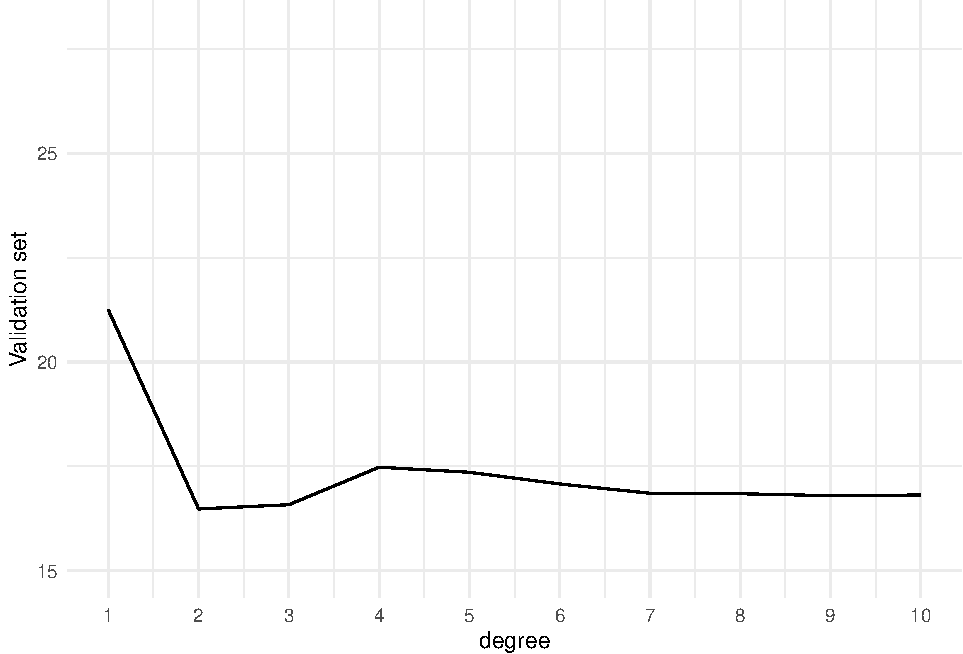
\includegraphics{3LinRegBEAMER_files/figure-beamer/unnamed-chunk-1-1.pdf}

\end{frame}

\begin{frame}[fragile]

\textbf{Interesting questions}

\begin{enumerate}
\def\labelenumi{\arabic{enumi}.}
\tightlist
\item
  Is there a relationship between \texttt{rent} and \texttt{area}?
\item
  How strong is this relationship?
\item
  Is the relationship linear?
\item
  Are also other variables associated with \texttt{rent}?
\item
  How well can we predict the rent of an appartment?
\item
  Is the effect of \texttt{area} the same on \texttt{rent} for
  appartments at average, good and top \texttt{location}? (interaction)
\end{enumerate}

\end{frame}

\begin{frame}{Simple Linear Regression}

\begin{itemize}
\tightlist
\item
  One quantitative response \(Y\) is modelled with
\item
  from \emph{one covariate} \(x\) (=simple),
\item
  and the relationship between \(Y\) and \(x\) is assumed to be
  \emph{linear}.
\end{itemize}

\end{frame}

\begin{frame}

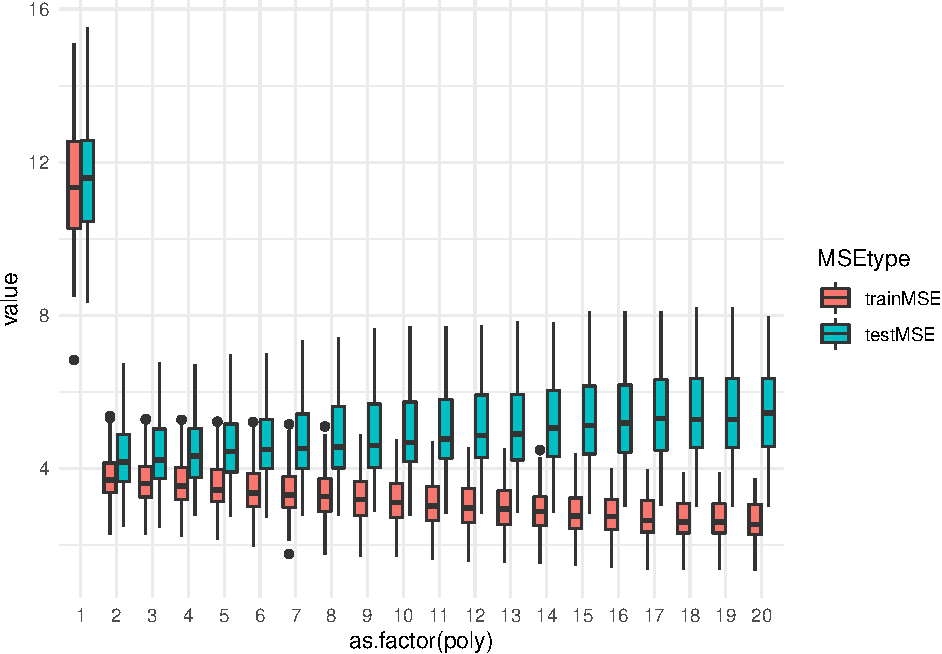
\includegraphics{3LinRegBEAMER_files/figure-beamer/unnamed-chunk-2-1.pdf}

\end{frame}

\begin{frame}

\begin{block}{Model and assumptions}

\[Y = f(x)+ \varepsilon= \beta_0 + \beta_1 x + \varepsilon\]

\begin{itemize}
\tightlist
\item
  \(Y\) is a \emph{quantitative} (continuous) response variable.
\item
  \(\beta_0\) is the \emph{intercept}. It is the average value of \(Y\)
  when \(x=0\).
\item
  \(\beta_1\) is the \emph{regression coefficient} or \emph{regression
  parameter} (slope). The slope represents the average increase in \(Y\)
  given a one-unit increase in \(x\).
\item
  \(x\) is the covariate. It can be continuous or discrete.
\item
  \(\varepsilon\) is the \emph{error term} also called the measurement
  noise. It replaces all the unobserved covariates that influence \(Y\).

  \begin{itemize}
  \tightlist
  \item
    \(\text{E}(\varepsilon)=0\)
  \item
    \(\text{Var}(\varepsilon)=\sigma^2\) (for all \(x\)).
  \item
    Often we also assume that \(\varepsilon\) is normally distributed.
  \end{itemize}
\end{itemize}

Here the \emph{model parameters} \(\beta_0\), \(\beta_1\) and
\(\sigma^2\) are unknown and have to be estimated from \emph{observed
data}.

\end{block}

\end{frame}

\begin{frame}

\begin{block}{Estimation and prediction}

\begin{itemize}
\tightlist
\item
  \emph{Fitting} a model is to find the best estimates for the model
  parameters.
\item
  This is based on data: independent pairs \((x_i,Y_i)\),
  \(i=1,\ldots,n\).
\item
  The \emph{least squares method} is used.
\item
  We can predict the value of the response for a (new) observation of
  the covariate at \(x_0\).
  \[\hat{Y} = \hat{\beta}_0 + \hat{\beta_1}x_0.\]
\end{itemize}

We use the \(\hat{}\) symbol for estimated or predicted values.

\end{block}

\end{frame}

\begin{frame}[fragile]

\begin{block}{Example continued: Munich rent index}

Assume a linear relationship between the monthly net rent
(\texttt{rent}) and the living area (\texttt{area}) in square meters.

In R: fit simple linear regression model using the \texttt{lm} function
to the data, and plot the data together with the \emph{fitted model}.

\begin{verbatim}
## (Intercept)        area 
##  134.592194    4.821464
\end{verbatim}

\end{block}

\end{frame}

\begin{frame}[fragile]

We see that the model fits the data quite well. It captures the essence.
It looks that a linear relationship between the response \texttt{rent}
and covariate \texttt{area} is a good approximation.

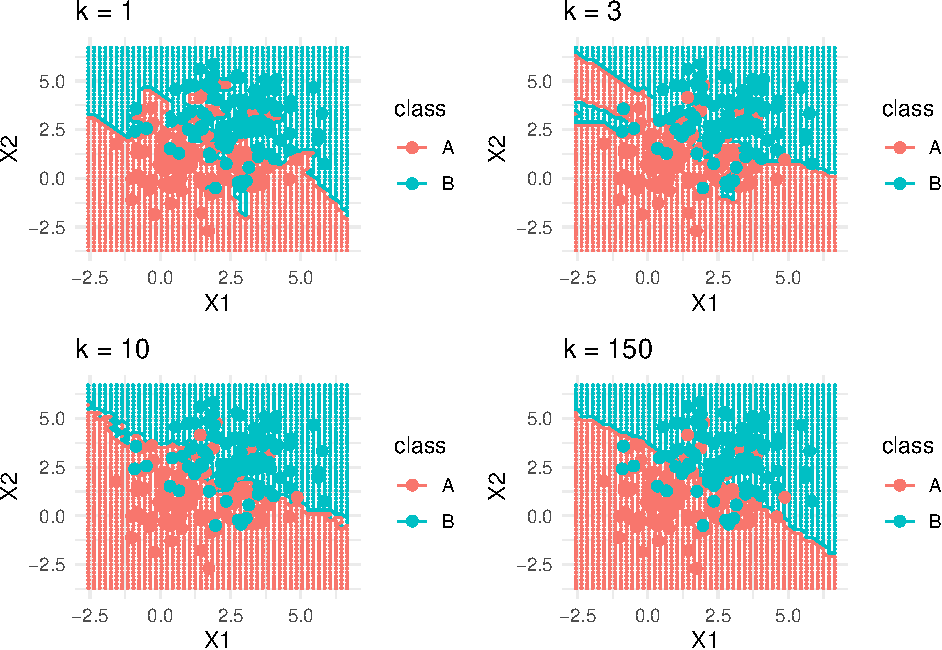
\includegraphics{3LinRegBEAMER_files/figure-beamer/unnamed-chunk-4-1.pdf}

\end{frame}

\begin{frame}

\textbf{Q:}

\begin{itemize}
\tightlist
\item
  The blue line gives the estimated model. Explain what the line means
  in practice.
\item
  How does this relate to the \emph{true} (population) model?
\item
  The spread around the fit does not look constant. What does this mean?
  Is that a problem?
\end{itemize}

\end{frame}

\begin{frame}[fragile]

\textbf{A}:

\begin{itemize}
\tightlist
\item
  If we compare two appartments where one has area 1 sq metre more then
  the other, we would expect the rent to be \(\hat{\beta}_1\) Euro
  higher.
\item
  The true model: tja, might also be approximately linear on the
  population level (all appartments in Munich), and it might be
  different from the blue line. To give the population level
  \texttt{area} vs \texttt{rent} we need to plot the relationship
  between all units in the population - and if we assume the
  relationship is linear that line might deviate from our blue line.
\item
  Yes, in linear regression we assume the variance of \(\varepsilon\) to
  be constant - the same for appartments of any \texttt{area}.
\end{itemize}

\end{frame}

\begin{frame}

\begin{block}{Parameter estimates: least squares}

Assume that we have a data set consisting of \(n\) observation pairs
\((x_i, Y_i)\) for \(i = 1,2,..., n\). We usually assume the \emph{pairs
are independent}.

Further, assume we fit a linear model to our data. For a single pair of
observations \((x_i, Y_i)\) it can be written as
\(\hat{Y}_i = \hat{\beta}_0 + \hat{\beta}_1 x_i\).

The \(i\)-th \emph{residual} of the model is the difference between the
\(i\)-th \emph{observed} response value and the \(i\)-th
\emph{predicted} value, and is written as: \[e_i = Y_i - \hat{Y}_i.\]

We may regard the residuals as \emph{predictions} (not estimates) of the
error terms \(\varepsilon_i\).

Remark: the error terms are random variables and can not be estimated -
they can be predicted. (It is only for parameters we find parameter
estimates.)

\end{block}

\end{frame}

\begin{frame}

The \emph{residual sum of squares (RSS)} is the squared sum of all
residuals
\[\begin{aligned} \text{RSS} &= e_1^2+e_2^2+...+e_n^2 \\ &= (Y_1 - \hat{\beta}_0 - \hat{\beta}_1 x_1)^2  + (Y_2 -\hat{\beta}_0 - \hat{\beta}_1 x_2)^2+ ... + (Y_n -\hat{\beta}_0 - \hat{\beta}_1 x_n)^2  \end{aligned}\]

We find the parameter estimates for \(\beta_0\) and \(\beta_1\) by
minimizing the RSS.

\textbf{Least squares estimators:}

\[\hat{\beta}_0 = \bar{Y}-\hat{\beta}_1 \bar{x}\] and
\[\hat{\beta}_1 = \frac{\sum_{i=1}^n(x_i-\bar{x})(Y_i-\bar{Y})}{\sum_{i=1}^n(x_i-\bar{x})^2},\]
where \(\bar{Y} = \frac{1}{n} \sum_{i=1}^n Y_i\) and
\(\bar{x} = \frac{1}{n}\sum_{i=1}^n x_i\) are the sample means.

\end{frame}

\begin{frame}[fragile]

\begin{block}{Example continued}

The coefficient estimates from our simple linear model fit to the Munich
rent index data can be printed using the \texttt{coef} function in R:

\begin{Shaded}
\begin{Highlighting}[]
\KeywordTok{coef}\NormalTok{(munich1.lm)}
\end{Highlighting}
\end{Shaded}

\begin{verbatim}
## (Intercept)        area 
##  134.592194    4.821464
\end{verbatim}

\textbf{Q}: Explain what these two values mean.

\end{block}

\end{frame}

\begin{frame}

\begin{block}{Accuracy of the parameter estimates}

(We will \emph{derive a general version} of these formulas for multiple
linear regression, because without matrix notation this is very
cumbersome - e.g.
\href{https://wiki.math.ntnu.no/tma4245/tema/begreper/regression}{``Egenskaper
til estimatorene'' for the TMA4240/TMA4245 Thematic pages}.)

The standard errors of the estimates are given by the following
formulas:
\[\text{Var}(\hat{\beta}_0)=\text{SE}(\hat{\beta}_0)^2 = \sigma^2 \Big [ \frac{1}{n} + \frac{\bar{x}^2}{\sum_{i=1}^n (x_i -\bar{x})^2} \Big]\]
and
\[\text{Var}(\hat{\beta}_1)=\text{SE}(\hat{\beta}_1)^2 = \frac{\sigma^2}{\sum_{i=1}^n (x_i-\bar{x})^2}.\]
In addition \(\text{Cov}(\hat{\beta_0},\hat{\beta_1})\) is in general
different from zero.

\end{block}

\end{frame}

\begin{frame}

We see how the estimated coefficient will vary when our experiment is
repeated.

Remark: SE=standard error vs SD=standard deviation - since we write SE
of a random variable this means the standard deviation of this variable
(square root of variance) - so for us SD and SE will be the same.

In general much confusion about SD and SE in articles:
\url{https://www.ncbi.nlm.nih.gov/pmc/articles/PMC1255808/}

\end{frame}

\begin{frame}

\textbf{Q: The best design}

Assume that we know the value of \(\sigma^2\). Now, observe that

\[\text{SE}(\hat{\beta}_1)^2 = \frac{\sigma^2}{\sum_{i=1}^n (x_i-\bar{x})^2}\]
is only dependent on the \emph{design} of the \(x_i\)'s.

\begin{itemize}
\tightlist
\item
  Would we like the \(\text{SE}(\hat{\beta}_1)^2\) large or small? Why?
\item
  If it is possible for us to choose the \(x_i\)'s, which strategy
  should we use to choose them?
\item
  Assume \(x\) can take values from 1 to 10 and we choose \(n=10\)
  values. Which is the best design?

  \begin{itemize}
  \tightlist
  \item
    evenly in a grid: \([1,2,3,4,5,6,7,8,9,10]\).
  \item
    only lower and upper value: \([1,1,1,1,1,10,10,10,10,10]\).
  \item
    randomly drawn from a uniform distribution on \([1,10]\).
  \end{itemize}
\end{itemize}

\end{frame}

\begin{frame}[fragile]

\begin{Shaded}
\begin{Highlighting}[]
\NormalTok{x1 =}\StringTok{ }\KeywordTok{seq}\NormalTok{(}\DecValTok{1}\OperatorTok{:}\DecValTok{10}\NormalTok{)}
\NormalTok{x2 =}\StringTok{ }\KeywordTok{c}\NormalTok{(}\KeywordTok{rep}\NormalTok{(}\DecValTok{1}\NormalTok{, }\DecValTok{5}\NormalTok{), }\KeywordTok{rep}\NormalTok{(}\DecValTok{10}\NormalTok{, }\DecValTok{5}\NormalTok{))}
\NormalTok{x3 =}\StringTok{ }\KeywordTok{runif}\NormalTok{(}\DecValTok{10}\NormalTok{, }\DecValTok{1}\NormalTok{, }\DecValTok{10}\NormalTok{)}

\NormalTok{sd1 =}\StringTok{ }\KeywordTok{sqrt}\NormalTok{(}\DecValTok{1}\OperatorTok{/}\KeywordTok{sum}\NormalTok{((x1 }\OperatorTok{-}\StringTok{ }\KeywordTok{mean}\NormalTok{(x1))}\OperatorTok{^}\DecValTok{2}\NormalTok{))}
\NormalTok{sd2 =}\StringTok{ }\KeywordTok{sqrt}\NormalTok{(}\DecValTok{1}\OperatorTok{/}\KeywordTok{sum}\NormalTok{((x2 }\OperatorTok{-}\StringTok{ }\KeywordTok{mean}\NormalTok{(x2))}\OperatorTok{^}\DecValTok{2}\NormalTok{))}
\NormalTok{sd3 =}\StringTok{ }\KeywordTok{sqrt}\NormalTok{(}\DecValTok{1}\OperatorTok{/}\KeywordTok{sum}\NormalTok{((x3 }\OperatorTok{-}\StringTok{ }\KeywordTok{mean}\NormalTok{(x3))}\OperatorTok{^}\DecValTok{2}\NormalTok{))}

\KeywordTok{print}\NormalTok{(}\KeywordTok{c}\NormalTok{(sd1, sd2, sd3))}
\end{Highlighting}
\end{Shaded}

\begin{verbatim}
## [1] 0.11009638 0.07027284 0.11512750
\end{verbatim}

\end{frame}

\begin{frame}

\textbf{A}: the second design - all observations at extremes.

\end{frame}

\begin{frame}

\begin{block}{Residual standard error}

Remember - residual sum of squares:
\(\text{RSS}=\sum_{i=1}^n (Y_i-\hat{\beta}_0-\hat{\beta_1}x_{i})^2\).

The residual standard error, RSE, is given by
\[\text{RSE}  =\sqrt{\frac{1}{n-2} \text{RSS}} = \sqrt{\frac{1}{n-2}\sum_{i=1}^n (Y_i -\hat{Y}_i)^2}\]
and is an estimate of \(\sigma\), that is, the standard deviation of the
error term \(\varepsilon\). This is the socalled \emph{restricted
maximum likelihood estimator}, and is unbiased.

This is related to the amount the response variables deviate from the
estimated regression line. Recall that we will always have observations
with noise.

RSE shows the lack of fit of the model to the data. It is measured in
units of \(Y\), hence is value may be hard to interpret.

\end{block}

\end{frame}

\begin{frame}[fragile]

If we assume that the simple linear regression is a good model,
observation pairs \((x_i,Y_i)\) are independent for \(i=1,\ldots,n\) and
that \(\varepsilon_i\sim N(0,\sigma^2)\) then it can be shown that

\[\frac{\text{RSE}^2(n-2)}{\sigma^2}= \frac{\sum_{i=1}^n (Y_i -\hat{Y}_i)^2}{\sigma^2}\sim \chi^2_{n-2}\]

\begin{block}{Example continued}

In R we can get a summary of our fitted linear model, by calling the
\texttt{summary} function. In this outprint we see the estimated
coefficient values in the first column, and the estimated standard
errors in the second column. Thus
\(\hat{\text{SE}}(\hat{\beta}_0) = 8.6135\) and
\(\hat{\text{SE}}(\hat{\beta}_1) = 0.1206\).

\end{block}

\end{frame}

\begin{frame}[fragile]

\small

\begin{Shaded}
\begin{Highlighting}[]
\KeywordTok{summary}\NormalTok{(munich1.lm)}
\end{Highlighting}
\end{Shaded}

\begin{verbatim}
## 
## Call:
## lm(formula = rent ~ area, data = rent99)
## 
## Residuals:
##     Min      1Q  Median      3Q     Max 
## -786.63 -104.88   -5.69   95.93 1009.68 
## 
## Coefficients:
##             Estimate Std. Error t value Pr(>|t|)    
## (Intercept) 134.5922     8.6135   15.63   <2e-16 ***
## area          4.8215     0.1206   39.98   <2e-16 ***
## ---
## Signif. codes:  0 '***' 0.001 '**' 0.01 '*' 0.05 '.' 0.1 ' ' 1
## 
## Residual standard error: 158.8 on 3080 degrees of freedom
## Multiple R-squared:  0.3417, Adjusted R-squared:  0.3415 
## F-statistic:  1599 on 1 and 3080 DF,  p-value: < 2.2e-16
\end{verbatim}

\normalsize

\end{frame}

\begin{frame}

To illustrate this point further, we fit four models to our Munich rent
index data set. Each of the models has been fit using a random sample of
a fraction of our observations (1/4). We see how our fitted line changes
given a ``new'' set of observations.

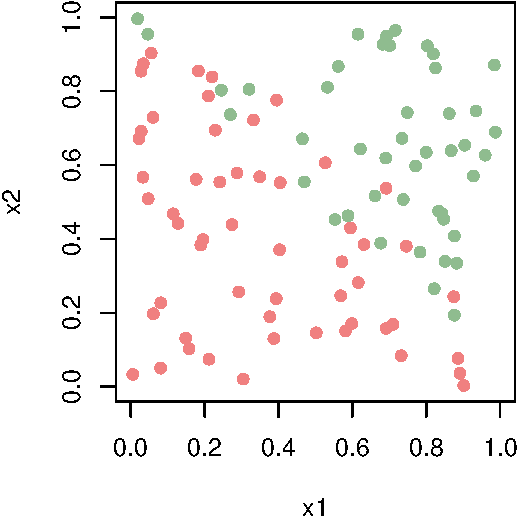
\includegraphics{3LinRegBEAMER_files/figure-beamer/unnamed-chunk-9-1.pdf}

\end{frame}

\begin{frame}

\begin{block}{Distribution of parameter estimators}

(We will \emph{derive a general version} for multiple linear
regression.)

For \(j=0,1\):

\begin{itemize}
\tightlist
\item
  Let \(\hat{\beta_j}\) be the least squares estimator for \(\beta_j\),
  and
\item
  \(\text{Var}(\hat{\beta_j})\) and
  \(\widehat{\text{Var}}(\hat{\beta_j})\) is as given above.
\end{itemize}

Then \(\hat{\beta}_j \sim N(\beta_j,\text{Var}(\hat{\beta}_j))\) and
\[T_j =\frac{\hat{\beta}_j-\beta_j}{\sqrt{\widehat{\text{Var}}(\hat{\beta}_j)}} \sim t_{n-2}\]
The \(t\)-distribution with \(n-2\) degrees of freedom.

See
\href{https://wwww.math.ntnu.no/emner/TMA4268/2018v/1Intro/Rintermediate-sol.html}{Rintermediate-sol.html}
for more on the \(t\)-distribution in R.

For the slope in the simple linear regression this is shown, together
with inference for \(\beta_1\), in this
\href{https://mediasite.ntnu.no/Mediasite/Play/2e9a209c58874e75bd47e3c5e0b7b4e81d?catalog=0fce6173-7a98-4db7-84b7-50cba3a3a341}{video
from TMA4240/TMA4245 Statistics (in Norwegian - but formulas should
still be understood in English).}

\end{block}

\end{frame}

\begin{frame}

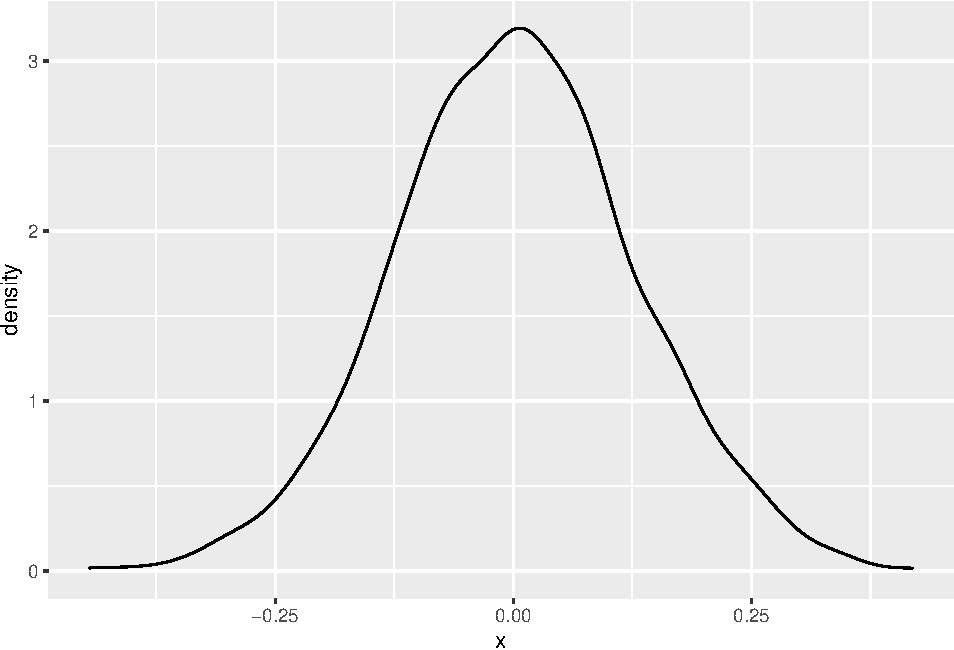
\includegraphics{3LinRegBEAMER_files/figure-beamer/unnamed-chunk-10-1.pdf}

The figure shows the \(t_{10}\) distribution, where the points were the
area under the curve to the right and left are with \(\alpha/2=0.025\).

\end{frame}

\begin{frame}[fragile]

\begin{block}{Confidence intervals}

The \(t\)-distribution can be used to create confidence intervals for
the regression parameters. The lower and upper limits of a 95\%
confidence interval for \(\beta_j\) are
\[\hat{\beta}_j \pm t_{\alpha/2,n-2} \cdot\text{SE} (\hat{\beta}_j) \quad j=0, 1.\]
The interpretation of this confidence is that: (before we have
contructed the interval) there is a 95\% chance that the interval will
contain the \emph{true} value of \(\beta_j\).

If \(n\) is large, the normal approximation to the \(t\)-distribution
can be used (and is used in the textbook).

\textbf{Q:} Calculate the confidence intervals for the slope parameter
in the \texttt{munich1.lm} model by finding the numbers you need from
the \texttt{summary} output. Here \(t_{0.025,n-2}\)=1.961.

\end{block}

\end{frame}

\begin{frame}[fragile]

We can find confidence intervals in \texttt{R} using the
\texttt{confint} function on \texttt{lm} object:

\begin{Shaded}
\begin{Highlighting}[]
\KeywordTok{confint}\NormalTok{(munich1.lm)}
\end{Highlighting}
\end{Shaded}

\begin{verbatim}
##                  2.5 %     97.5 %
## (Intercept) 117.703417 151.480972
## area          4.585017   5.057912
\end{verbatim}

Remark: the argument \texttt{level=0.99} will give a 99\% CI.

Based on the joint distribution of the intercept and slope it is
possible to find the distribution for the linear predictor
\(\hat{\beta}_0+\hat{\beta}_1 x\), and then confidence intervals for
\(\beta_0+\beta_1 x\).

\end{frame}

\begin{frame}

\includegraphics{3LinRegBEAMER_files/figure-beamer/unnamed-chunk-12-1.pdf}

The figures show the fitted line and the confidence interval for the
(true) regression line based on all (left) and the first 100
observations (right) in the Munich rent index data. Observe the effect
of the sample size on the with of the CIs.

\end{frame}

\begin{frame}

\begin{block}{Single hypothesis testing set-up}

In single hypothesis testing we are interesting in testing one null
hypothesis against an alternative hypothesis. In linear regression the
hypothesis is often about a regression parameter \(\beta_j\):
\[H_0: \beta_j=0 \text{ vs. } H_1: \beta_j\neq 0\]

\begin{block}{Two types of errors:}

\begin{itemize}
\item
  ``Reject \(H_0\) when \(H_0\) is true''=``false positives'' = ``type I
  error'' =``miscarriage of justice''. These are our \emph{fake news},
  which are very important for us to avoid.
\item
  ``Fail to reject \(H_0\) when \(H_1\) is true (and \(H_0\) is
  false)''=``false negatives'' = ``type II error''= ``guilty criminal go
  free''.
\end{itemize}

\end{block}

\end{block}

\end{frame}

\begin{frame}

We choose to reject \(H_0\) at some significance level \(\alpha\) if the
\(p\)-value of the test (see below) is smaller than the chosen
significance level. We say that : Type I error is ``controlled'' at
significance level \(\alpha\), which means that the probability of
miscarriage of justice (Type I error) does not exceed \(\alpha\).

\textbf{Q}: Draw a 2 by 2 table showing the connection between

\begin{itemize}
\tightlist
\item
  ``truth'' (\(H_0\) true or \(H_0\) false) - rows in the table, and
\item
  ``action'' (reject \(H_0\) and accept \(H_0\)) - columns in the table,
\end{itemize}

and place the two types of errors in the correct position within the
table.

What else should be written in the last two cells?

\end{frame}

\begin{frame}

\begin{block}{Hypothesis test on \(\beta_j\) (t-test)}

In linear regression models our test statistic for testing
\(H_0: \beta_j=0\) is
\[T_0=\frac{\hat{\beta}_j-0}{\sqrt{c_{jj}}\hat{\sigma}_{\varepsilon}}\sim t_{n-2}\]
where
\(c_{jj}\hat{\sigma}_{\varepsilon}^2=\widehat{\text{Var}}(\hat{\beta}_j)\).

Inserted observed values (and estimates) we have \(t_0\).

We would in a two-sided setting reject \(H_0\) for large values of
\(\text{abs}(t_0)\). We may rely on calculating a \(p\)-value.

\end{block}

\end{frame}

\begin{frame}

\begin{block}{The p-value}

A p-value is a test statistic satisfying \(0 \leq p({\bf Y}) \leq 1\)
for every vector of observations \({\bf Y}\).

\begin{itemize}
\item
  Small values give evidence that \(H_1\) is true.
\item
  In single hypothesis testing, if the p-value is less than the chosen
  significance level (chosen upper limit for the probability of
  committing a type I error), then we reject the null hypothesis,
  \(H_0\). The chosen significance level is often referred to as
  \(\alpha\).
\item
  A p-value is \emph{valid} if
  \[ P(p({\bf Y}) \leq \alpha) \leq \alpha\] for all \(\alpha\),
  \(0 \leq \alpha \leq 1\), whenever \(H_0\) is true, that is, if the
  \(p\)-value is valid, rejection on the basis of the \(p\)-value
  ensures that the probability of type I error does not exceed
  \(\alpha\).
\item
  If \(P(p({\bf Y}) \leq \alpha) = \alpha\) for all \(\alpha\),
  \(0 \leq \alpha \leq 1\), the \(p\)-value is called an \emph{exact}
  p-value.
\end{itemize}

\end{block}

\end{frame}

\begin{frame}

In our linear regression we use the \(t\)-distibution to calculate
p-values for our two-sided test situation \(H_0: \beta_j=0\) vs.
\(H_1: \beta_j \neq 0\). Assume we have observed that our test statistic
\(T_0\) takes the numerical value \(t_0\). Since the \(t\)-distribution
is symmetric around \(0\) we have

\[p\text{-value}=P(T_0>\text{abs}(t_0))+P(T_0<-\text{abs}(t_0))=2\cdot P(T_0>\text{abs}(t_0)).\]

We reject \(H_0\) if our calculated \(p\)-value is below our chosen
signficance level. We often choose as significance level
\(\alpha=0.05\).

\end{frame}

\begin{frame}[fragile]

\textbf{Q:} Comment on the \(p\)-values listed in the summary output
from fitting the simple linear regression of \texttt{area} and
\texttt{rent}. Then, pinpoint \(\hat{\sigma}_{\varepsilon}=\text{RSE}\).
Where are the entries in the output that you do not (yet) know what is?

\footnotesize

\begin{verbatim}
## 
## Call:
## lm(formula = rent ~ area, data = rent99)
## 
## Residuals:
##     Min      1Q  Median      3Q     Max 
## -786.63 -104.88   -5.69   95.93 1009.68 
## 
## Coefficients:
##             Estimate Std. Error t value Pr(>|t|)    
## (Intercept) 134.5922     8.6135   15.63   <2e-16 ***
## area          4.8215     0.1206   39.98   <2e-16 ***
## ---
## Signif. codes:  0 '***' 0.001 '**' 0.01 '*' 0.05 '.' 0.1 ' ' 1
## 
## Residual standard error: 158.8 on 3080 degrees of freedom
## Multiple R-squared:  0.3417, Adjusted R-squared:  0.3415 
## F-statistic:  1599 on 1 and 3080 DF,  p-value: < 2.2e-16
\end{verbatim}

\normalsize

\end{frame}

\begin{frame}

\begin{block}{Model accuracy}

\begin{block}{Coefficient of determination, \(R^2\)}

The total sum of squares is defined as
\[\text{TSS} = \sum_{i=1}^n (y_i - \bar{y})^2,\] and is proportional to
the estimated variance of the response variable.

The \(R^2\) statisitic is the fraction of variance explained by the
model and is given by
\[R^2 = \frac{\text{TSS}-\text{RSS}}{TSS}= 1-\frac{\text{RSS}}{\text{TSS}}=1-\frac{\sum_{i=1}^n(y_i-\hat{y}_i)^2}{\sum_{i=1}^n(y_i-\bar{y}_i)^2}.\]
The value is between 0 and 1, and we want an as high \(R^2\) statistic
as possible. This statistic is independent of the scale of \(Y\).

\end{block}

\end{block}

\end{frame}

\begin{frame}[fragile]

For a simple linear regression model the squared correlation \(r^2\) is
equal to \(R^2\).

\textbf{Q}: Look back at the \texttt{summary} outprint for the
\texttt{munich1.lm} model. What is the value of the \(R^2\) statistic?
Based on this value, would you conclude that this model gives a good fit
to the data?

\end{frame}

\begin{frame}[fragile]{Multiple Linear Regression}

Back to the Munich rent index data, but now we want to include more than
one covariate. Suggestions?

\begin{itemize}
\tightlist
\item
  \texttt{rent}: the net rent per month (in Euro).
\item
  \texttt{rentsqm}: the net rent per month per square meter (in Euro).
\item
  \texttt{area}: Living area in square meters.
\item
  \texttt{yearc}: year of construction.
\item
  \texttt{location}: quality of location: a factor indicating whether
  the location is average location, 1, good location, 2, and top
  location, 3.
\item
  \texttt{bath}: quality of bathroom: a a factor indicating whether the
  bath facilities are standard, 0, or premium, 1.
\item
  \texttt{kitchen}: Quality of kitchen: 0 standard 1 premium.
\item
  \texttt{cheating}: central heating: a factor 0 without central
  heating, 1 with central heating.
\item
  \texttt{district}: District in Munich.
\end{itemize}

\end{frame}

\begin{frame}

\begin{block}{Model}

We assume, for observation \(i\):
\[Y_i= \beta_0 + \beta_{1}  x_{i1} + \beta_2 x_{i2} + ... + \beta_p x_{ip} + \varepsilon_i,\]
where \(i=1,2,...,n\).

Here: what is \(x_{ij}\)?

The model can be written in matrix form:
\[{\bf Y}={\bf X} \boldsymbol{\beta}+{\boldsymbol{\varepsilon}}.\]

\textbf{Q}: write out in detail the dimension!

\end{block}

\end{frame}

\begin{frame}

\begin{block}{Notation}

\({\bf Y}: (n \times 1)\) vector of responses {[}e.g.~one of the
following: rent, weight of baby, ph of lake, volume of tree{]}

\({\bf X}: (n \times (p+1))\) design matrix {[}e.g.~location of flat,
gestation age of baby, chemical measurement of the lake, height of
tree{]}, and \({\bf x}_i^T\) is a \((p+1)\)-dimensional row row vector
for observation \(i\).

\({\boldsymbol \beta}: ((p+1) \times 1)\) vector of regression
parameters (intercept included)

\({\boldsymbol \varepsilon}: (n\times 1)\) vector of random errors.

We assume that pairs \(({\bf x}_i^T,y_i)\) \((i=1,...,n)\) are measured
from sampling units. That is, the observation pair \(({\bf x}_1^T,y_1)\)
is independent from \(({\bf x}_2^T,y_2)\).

Remark: other books, including the book in TMA4267 and TMA4315 define
\(p\) to include the intercept. This may lead to some confusion about
\(p\) or \(p+1\) in formulas\ldots{}

\end{block}

\end{frame}

\begin{frame}[fragile]

\begin{block}{Example continued}

Assume that we have \texttt{rent} as response and \texttt{area} and
\texttt{bath} as covariates.

\begin{itemize}
\tightlist
\item
  What is \({\bf Y}\), \({\bf X}\), \(\boldsymbol{\beta}\) and
  \(\boldsymbol{\varepsilon}\)?
\item
  Which of these are known/unknown, observed/unobserved?
\end{itemize}

Remember: \(n=3802\) and \texttt{bath=0} gives standard quality and
\texttt{bath=1} premium and the model is
\[{\bf Y=X \boldsymbol\beta}+{\boldsymbol \varepsilon}.\]

\end{block}

\end{frame}

\begin{frame}[fragile]

\small

\begin{Shaded}
\begin{Highlighting}[]
\NormalTok{fit =}\StringTok{ }\KeywordTok{lm}\NormalTok{(rent }\OperatorTok{~}\StringTok{ }\NormalTok{area }\OperatorTok{+}\StringTok{ }\NormalTok{bath, }\DataTypeTok{data =}\NormalTok{ rent99)}
\KeywordTok{head}\NormalTok{(}\KeywordTok{model.matrix}\NormalTok{(fit))}
\end{Highlighting}
\end{Shaded}

\begin{verbatim}
##   (Intercept) area bath1
## 1           1   26     0
## 2           1   28     0
## 3           1   30     0
## 4           1   30     0
## 5           1   30     0
## 6           1   30     0
\end{verbatim}

\begin{Shaded}
\begin{Highlighting}[]
\KeywordTok{head}\NormalTok{(rent99}\OperatorTok{$}\NormalTok{rent)}
\end{Highlighting}
\end{Shaded}

\begin{verbatim}
## [1] 109.9487 243.2820 261.6410 106.4103 133.3846 339.0256
\end{verbatim}

\normalsize

\end{frame}

\begin{frame}

\begin{block}{Classical linear model}

Assumptions:

\begin{enumerate}
\def\labelenumi{\arabic{enumi}.}
\tightlist
\item
  \(\text{E}(\boldsymbol{\varepsilon})=\bf{0}\).
\item
  \(\text{Cov}(\boldsymbol{\varepsilon})=\text{E}(\boldsymbol{\varepsilon}\boldsymbol{\varepsilon}^T)=\sigma^2\bf{I}\).
\item
  The design matrix has full rank, \(\text{rank}({\bf X})=p+1\). (We
  assume \(n>>(p+1)\).)
\end{enumerate}

The classical \emph{normal} linear regression model is obtained if
additionally

\begin{enumerate}
\def\labelenumi{\arabic{enumi}.}
\setcounter{enumi}{3}
\tightlist
\item
  \(\boldsymbol\varepsilon\sim N_n({\bf 0},\sigma^2 {\bf I})\) holds.
  Here \(N_n\) denotes the \(n\)-dimensional multivarate normal
  distribution.
\end{enumerate}

For random covariates these assumptions are to be understood
conditionally on \({\bf X}\).

The interpretation of the coefficients \(\beta_j\) is now as following:
holding all other covariates fixed, what is the average effect on \(Y\)
of a one-unit increase in the \(j\)th covariate.

\end{block}

\end{frame}

\begin{frame}

\begin{block}{Distribution of the response vector}

Assume that \({\bf Y=X \boldsymbol\beta}+{\boldsymbol \varepsilon}\) and
\(\boldsymbol\varepsilon\sim N_n({\bf 0},\sigma^2 {\bf I})\).

\textbf{Q:}

\begin{itemize}
\tightlist
\item
  Find the mean \(\text{E}(\bf Y)\) and
\item
  the covariance matrix \(\text{Cov}(\bf Y)\).
\item
  What is then the distribution of \(\bf Y\)?
\end{itemize}

\end{block}

\end{frame}

\begin{frame}

\textbf{A}:
\[ {\bf Y} \sim N_{n}({\bf X} {\boldsymbol\beta},\sigma^2 {\bf I})\]

\end{frame}

\begin{frame}

\begin{block}{Parameter estimation}

In multiple linear regression parameters in \(\beta\) are estimated with
maximum likelihood and least squares. These two methods give the same
estimator when we assume the normal linear regression model.

\textbf{Least squares and maximum likelihood estimator for
\({\bf \beta}\):}
\[ \hat{\boldsymbol\beta}=({\bf X}^T{\bf X})^{-1} {\bf X}^T {\bf Y}\]

\end{block}

\end{frame}

\begin{frame}

The estimator is found by minimizing the RSS for a multiple linear
regression model:
\[\begin{aligned} \text{RSS} &=\sum_{i=1}^n (y_i - \hat y_i)^2 = \sum_{i=1}^n (y_i - \hat \beta_0 - \hat \beta_1 x_{i1} - \hat \beta_2 x_{i2} -...-\hat \beta_p x_{ip} )^2 \\
&= \sum_{i=1}^n (y_i-{\bf x}_i^T \boldsymbol \beta)^2=({\bf Y}-{\bf X}\hat{\boldsymbol{\beta}})^T({\bf Y}-{\bf X}\hat{\boldsymbol{\beta}})\end{aligned}\]
The estimator is found by solving the system of (p+1) equation
:\(\frac{\partial \text{RSS}}{\partial \boldsymbol \beta}={\bf 0}\), see
\href{https://www.math.ntnu.no/emner/TMA4268/2018v/notes/LeastSquaresMLR.pdf}{LeastSquaresMLR.pdf}
for a derivation (from TMA4267V2017).

\end{frame}

\begin{frame}[fragile]

\begin{block}{Example continued}

Write down the model and explain what the values under \texttt{Estimate}
mean in practice.

\end{block}

\end{frame}

\begin{frame}[fragile]

\footnotesize

\begin{Shaded}
\begin{Highlighting}[]
\NormalTok{munich3.lm =}\StringTok{ }\KeywordTok{lm}\NormalTok{(rentsqm }\OperatorTok{~}\StringTok{ }\NormalTok{area }\OperatorTok{+}\StringTok{ }\NormalTok{yearc }\OperatorTok{+}\StringTok{ }\NormalTok{location }\OperatorTok{+}\StringTok{ }\NormalTok{bath }\OperatorTok{+}\StringTok{ }\NormalTok{kitchen }\OperatorTok{+}\StringTok{ }
\StringTok{    }\NormalTok{cheating, }\DataTypeTok{data =}\NormalTok{ rent99)}
\KeywordTok{summary}\NormalTok{(munich3.lm)}
\end{Highlighting}
\end{Shaded}

\begin{verbatim}
## 
## Call:
## lm(formula = rentsqm ~ area + yearc + location + bath + kitchen + 
##     cheating, data = rent99)
## 
## Residuals:
##     Min      1Q  Median      3Q     Max 
## -6.4303 -1.4131 -0.1073  1.3244  8.6452 
## 
## Coefficients:
##               Estimate Std. Error t value Pr(>|t|)    
## (Intercept) -45.475484   3.603775 -12.619  < 2e-16 ***
## area         -0.032330   0.001648 -19.618  < 2e-16 ***
## yearc         0.026959   0.001846  14.606  < 2e-16 ***
## location2     0.777133   0.076870  10.110  < 2e-16 ***
## location3     1.725068   0.236062   7.308 3.45e-13 ***
## bath1         0.762808   0.157559   4.841 1.35e-06 ***
## kitchen1      1.136908   0.183088   6.210 6.02e-10 ***
## cheating1     1.765261   0.129068  13.677  < 2e-16 ***
## ---
## Signif. codes:  0 '***' 0.001 '**' 0.01 '*' 0.05 '.' 0.1 ' ' 1
## 
## Residual standard error: 2.031 on 3074 degrees of freedom
## Multiple R-squared:  0.3065, Adjusted R-squared:  0.3049 
## F-statistic: 194.1 on 7 and 3074 DF,  p-value: < 2.2e-16
\end{verbatim}

\normalsize

\end{frame}

\begin{frame}[fragile]

Reproduce the values under \texttt{Estimate} by calculating without the
use of \texttt{lm}.

\begin{Shaded}
\begin{Highlighting}[]
\NormalTok{X =}\StringTok{ }\KeywordTok{model.matrix}\NormalTok{(rentsqm }\OperatorTok{~}\StringTok{ }\NormalTok{area }\OperatorTok{+}\StringTok{ }\NormalTok{yearc }\OperatorTok{+}\StringTok{ }\NormalTok{location }\OperatorTok{+}\StringTok{ }\NormalTok{bath }\OperatorTok{+}\StringTok{ }\NormalTok{kitchen }\OperatorTok{+}\StringTok{ }
\StringTok{    }\NormalTok{cheating, }\DataTypeTok{data =}\NormalTok{ rent99)}
\NormalTok{Y =}\StringTok{ }\NormalTok{rent99}\OperatorTok{$}\NormalTok{rentsqm}
\NormalTok{betahat =}\StringTok{ }\KeywordTok{solve}\NormalTok{(}\KeywordTok{t}\NormalTok{(X) }\OperatorTok\StringTok{ }\NormalTok{X) }\OperatorTok\StringTok{ }\KeywordTok{t}\NormalTok{(X) }\OperatorTok\StringTok{ }\NormalTok{Y}
\KeywordTok{print}\NormalTok{(betahat)}
\end{Highlighting}
\end{Shaded}

\begin{verbatim}
##                     [,1]
## (Intercept) -45.47548356
## area         -0.03233033
## yearc         0.02695857
## location2     0.77713297
## location3     1.72506792
## bath1         0.76280784
## kitchen1      1.13690814
## cheating1     1.76526110
\end{verbatim}

\end{frame}

\begin{frame}

\begin{block}{Distribution of the regression parameter estimator}

\begin{enumerate}
\def\labelenumi{\arabic{enumi}.}
\tightlist
\item
  We assumed that
  \({\bf Y=X \boldsymbol\beta}+{\boldsymbol \varepsilon}\) and
  \(\boldsymbol\varepsilon\sim N_n({\bf 0},\sigma^2 {\bf I})\), leading
  to \[ {\bf Y} \sim N_{n}(\bf X \boldsymbol \beta,\sigma^2 {\bf I}).\]
\item
  Then we ``found'' that an estimator for \({\bf \beta}\) is
  \[ \hat{\boldsymbol\beta}=({\bf X}^T{\bf X})^{-1} {\bf X}^T {\bf Y}.\]
\item
  From Module 2: Part B: \(\mathbf{Y}_{(n\times 1)}\) with mean vector
  \(\mathbf{\mu}\) and variance-covariance matrix \(\Sigma\), then
  \(\mathbf{Z}=\mathbf{C}\mathbf{Y}\) has
  \(\text{E}(\mathbf{Z})=\mathbf{C}\mathbf{\mu}\) and
  \(\text{Cov}(\mathbf{Z})=  \mathbf{C}\Sigma\mathbf{C}^T\).
\item
  Also Module 2: Part B: If \({\bf Y}\) is multivariate normal, then
  also \(\mathbf{C}\mathbf{Y}\) is multivariate normal.
\end{enumerate}

\textbf{Q: Homework for the 2nd lecture}

\begin{itemize}
\tightlist
\item
  Find the mean \(\text{E}(\hat{\boldsymbol\beta})\) and the covariance
  matrix \(\text{Cov}(\hat{\boldsymbol\beta})\) by yourself.
\item
  What is then the distribution of \(\hat{\boldsymbol\beta}\)?
\end{itemize}

\end{block}

\end{frame}

\begin{frame}[fragile]

\large

\textbf{Part B: Multiple linear regression - continued!}

\normalsize

\begin{block}{Data sets}

\begin{block}{Munich rent index (as in Part A)}

Munich, 1999: 3082 observations on 9 variables.

\begin{itemize}
\tightlist
\item
  \texttt{rent}: the net rent per month (in Euro).
\item
  \texttt{rentsqm}: the net rent per month per square meter (in Euro).
\item
  \texttt{area}: Living area in square meters.
\item
  \texttt{yearc}: year of construction.
\item
  \texttt{location}: quality of location: a factor indicating whether
  the location is average location, 1, good location, 2, and top
  location, 3.
\item
  \texttt{bath}: quality of bathroom: a a factor indicating whether the
  bath facilities are standard, 0, or premium, 1.
\item
  \texttt{kitchen}: Quality of kitchen: 0 standard 1 premium.
\item
  \texttt{cheating}: central heating: a factor 0 without central
  heating, 1 with central heating.
\item
  \texttt{district}: District in Munich.
\end{itemize}

\end{block}

\end{block}

\end{frame}

\begin{frame}[fragile]

\begin{block}{Ozone}

New York, 1973: 111 observations of

\begin{itemize}
\tightlist
\item
  \texttt{ozone} : ozone concentration (ppm)
\item
  \texttt{radiation} : solar radiation (langleys)
\item
  \texttt{temperature} : daily maximum temperature (F)
\item
  \texttt{wind} : wind speed (mph)
\end{itemize}

\texttt{ozone} as our response variable and \texttt{temperature},
\texttt{wind} and `radiation as covariates.

First 6 observations in data set printed.

\end{block}

\end{frame}

\begin{frame}[fragile]

\begin{verbatim}
##   ozone radiation temperature wind
## 1    41       190          67  7.4
## 2    36       118          72  8.0
## 3    12       149          74 12.6
## 4    18       313          62 11.5
## 5    23       299          65  8.6
## 6    19        99          59 13.8
\end{verbatim}

\end{frame}

\begin{frame}

\begin{block}{Plan for part B}

\begin{itemize}
\tightlist
\item
  So far: simple linear regression - and multiple linear regression -
  model, estimators
\item
  Statistical inference

  \begin{itemize}
  \tightlist
  \item
    estimators and properties
  \item
    confidence intervals and hypothesis tests
  \item
    significance of regression: F-test
  \item
    prediction and prediction intervals
  \end{itemize}
\item
  Model assessement and selection

  \begin{itemize}
  \tightlist
  \item
    \(R^2\)
  \item
    subset selection
  \item
    diagnostic plots - studentized residuals and leverages
  \end{itemize}
\end{itemize}

\end{block}

\end{frame}

\begin{frame}

\begin{itemize}
\tightlist
\item
  Extensions and challenges (self study)

  \begin{itemize}
  \tightlist
  \item
    qualitative predictors: dummy coding (needed)
  \item
    non-additivity: including interactions (useful)
  \item
    projection matrices and geometry of least squares (optional)
  \end{itemize}
\item
  Important results in MLR
\item
  Summing up with team Kahoot!
\end{itemize}

\end{frame}

\begin{frame}[fragile]{Multiple linear regression (continued)}

\begin{block}{Model and parameter estimator (summing up)}

Model: \[{\bf Y}=\bf X \boldsymbol{\beta}+{\boldsymbol{\varepsilon}}\]
with full rank design matrix \({\bf X}\).

\small

\begin{Shaded}
\begin{Highlighting}[]
\KeywordTok{head}\NormalTok{(}\KeywordTok{model.matrix}\NormalTok{(ozone.lm))}
\end{Highlighting}
\end{Shaded}

\begin{verbatim}
##   (Intercept) temperature wind radiation
## 1           1          67  7.4       190
## 2           1          72  8.0       118
## 3           1          74 12.6       149
## 4           1          62 11.5       313
## 5           1          65  8.6       299
## 6           1          59 13.8        99
\end{verbatim}

\begin{Shaded}
\begin{Highlighting}[]
\KeywordTok{head}\NormalTok{(ozone}\OperatorTok{$}\NormalTok{ozone)}
\end{Highlighting}
\end{Shaded}

\begin{verbatim}
## [1] 41 36 12 18 23 19
\end{verbatim}

\normalsize

\end{block}

\end{frame}

\begin{frame}

Classical \emph{normal} linear regression model when
\[\boldsymbol{\varepsilon}\sim N_n({\bf 0},\sigma^2{\bf I}).\]

In Part A we found that :
\[ {\bf Y} \sim N_{n}({\bf X} {\boldsymbol\beta},\sigma^2 {\bf I})\]

Parameter of interest is \(\boldsymbol{\beta}\) and \(\sigma^2\) is a
nuisance (=parameter not of interest).

Using the least squares (and maximum likelihood) method the estimator
for \(\boldsymbol\beta\) is
\[ \hat\beta=({\bf X}^T{\bf X})^{-1} {\bf X}^T {\bf Y}\]

\end{frame}

\begin{frame}

How does this compare to simple linear regression? Not so easy to see a
connection!

\[\hat{\beta}_0 = \bar{Y}-\hat{\beta}_1 \bar{x} \text{ and } \hat{\beta}_1 = \frac{\sum_{i=1}^n(x_i-\bar{x})(Y_i-\bar{Y})}{\sum_{i=1}^n(x_i-\bar{x})^2},\]

\[ \hat\beta=({\bf X}^T{\bf X})^{-1} {\bf X}^T {\bf Y}\]

Often we use centered data (and also scaled) to ease interpretation. In
design of experiments often orthogonal columns of the design matrix is
chosen to get \({\bf X}^T{\bf X}\) to be diagonal, which leads to easier
interpretation and identifiability.

\end{frame}

\begin{frame}[fragile]

\begin{block}{Distribution of the regression parameter estimator
(summing up)}

\[ \hat{\boldsymbol\beta}=({\bf X}^T{\bf X})^{-1} {\bf X}^T {\bf Y}\]

This can be written as \(\hat{\boldsymbol\beta}={\bf C}{\bf Y}\) where

\begin{itemize}
\tightlist
\item
  \({\bf C}=({\bf X}^T{\bf X})^{-1} {\bf X}^T\)
\item
  \({\bf Y} \sim N_{n}({\bf X} {\boldsymbol\beta},\sigma^2 {\bf I})\).
\end{itemize}

Therefore

\begin{itemize}
\tightlist
\item
  \(\hat{\boldsymbol\beta}\) is multivariate normal (p+1) dimensions,
  with
\item
  \(\text{E}(\hat{\boldsymbol\beta})={\bf C}\text{E}({\bf Y})=({\bf X}^T{\bf X})^{-1} {\bf X}^T{\bf X} {\boldsymbol\beta}={\boldsymbol\beta}\)
\item
  \(\text{Cov}(\hat{\boldsymbol\beta})={\bf C}\text{Cov}({\bf Y}){\bf C}^T=({\bf X}^T{\bf X})^{-1} {\bf X}^T \sigma^2 {\bf I}(({\bf X}^T{\bf X})^{-1} {\bf X}^T)^T =({\bf X}^T{\bf X})^{-1} \sigma^2\).
\end{itemize}

So:
\(\hat{\beta}\sim N_{p+1}(\boldsymbol{\beta},\sigma^2({\bf X}^T{\bf X})^{-1})\).

\end{block}

\begin{block}{\href{https://www.math.ntnu.no/emner/TMA4268/2018v/notes/PropertiesBetahatMLR.pdf}{PropertiesBetahatMLR.pdf}
for a derivation.}

\(\hat{\beta}\sim N_{p+1}(\boldsymbol{\beta},\sigma^2({\bf X}^T{\bf X})^{-1})\).

\footnotesize

\begin{Shaded}
\begin{Highlighting}[]
\KeywordTok{coefficients}\NormalTok{(ozone.lm)}
\end{Highlighting}
\end{Shaded}

\begin{verbatim}
##  (Intercept)  temperature         wind    radiation 
## -64.23208116   1.65120780  -3.33759763   0.05979717
\end{verbatim}

\begin{Shaded}
\begin{Highlighting}[]
\KeywordTok{vcov}\NormalTok{(ozone.lm)}
\end{Highlighting}
\end{Shaded}

\begin{verbatim}
##              (Intercept)  temperature          wind     radiation
## (Intercept) 530.93558002 -5.503192281 -1.043562e+01  0.0266688733
## temperature  -5.50319228  0.064218138  8.034556e-02 -0.0015749279
## wind        -10.43562350  0.080345561  4.275126e-01 -0.0003442514
## radiation     0.02666887 -0.001574928 -3.442514e-04  0.0005371733
\end{verbatim}

\normalsize

\textbf{Q:} Explain what all these numbers are!

\end{block}

\end{frame}

\begin{frame}

\begin{block}{Estimator for \(\sigma^2\)}

\[\begin{aligned} \text{RSS} &=\sum_{i=1}^n (y_i - \hat y_i)^2 = \sum_{i=1}^n (y_i - \hat \beta_0 - \hat \beta_1 x_{i1} - \hat \beta_2 x_{i2} -...-\hat \beta_p x_{ip} )^2 \\
&= \sum_{i=1}^n (y_i-{\bf x}_i^T \hat{\boldsymbol \beta})^2=({\bf Y}-{\bf X}\hat{\boldsymbol{\beta}})^T({\bf Y}-{\bf X}\hat{\boldsymbol{\beta}})\end{aligned}\]

Restricted maximum likelihood estimator for \({\bf \sigma}^2\):
\[ \hat{\sigma}^2=\frac{1}{n-p-1}({\bf Y}-{\bf X}\hat{\boldsymbol\beta})^T({\bf Y}-{\bf X}\hat{\boldsymbol\beta})=\frac{\text{RSS}}{n-p-1}\]
with \(\frac{(n-p-1)\hat{\sigma}^2}{\sigma^2} \sim \chi^2_{n-p-1}\).

\end{block}

\end{frame}

\begin{frame}

\begin{block}{Distribution of regression parameters (contd.)}

\(\hat{\beta}\sim N_{p+1}(\boldsymbol{\beta},\sigma^2({\bf X}^T{\bf X})^{-1})\).

\begin{itemize}
\tightlist
\item
  unbiased
\item
  covariance matrix dependent on the design (and \(\sigma^2\))
\end{itemize}

Multicollinearity: columns in design matrix (that is, the covariates)
are correlated, which may lead to difficulty in ``identifying'' the
effect of each covariate on the response, and thus large variances (and
covariances) for the elements of \(\hat{\boldsymbol\beta}\).

The \emph{variance inflation factor (VIF)} is the ratio of the variance
of \(\hat{\beta}_j\) when fitting a model with the chosen covariates
divided by the variance of \(\hat{\beta}_j\) in a simple linear
regression.

\begin{itemize}
\tightlist
\item
  VIF=1: absence of collinearity
\item
  VIF exceeding 5 or 10 might be problematic.
\item
  Solution: drop a covariate (that do not add much since it is
  correlated with other covariates).
\end{itemize}

\end{block}

\end{frame}

\begin{frame}[fragile]

\small

\begin{Shaded}
\begin{Highlighting}[]
\NormalTok{oz1 =}\StringTok{ }\KeywordTok{as.data.frame}\NormalTok{(}\KeywordTok{apply}\NormalTok{(ozone, }\DecValTok{2}\NormalTok{, scale, }\DataTypeTok{scale =} \OtherTok{FALSE}\NormalTok{))}
\NormalTok{fitoz =}\StringTok{ }\KeywordTok{lm}\NormalTok{(ozone }\OperatorTok{~}\StringTok{ }\NormalTok{temperature }\OperatorTok{+}\StringTok{ }\NormalTok{wind }\OperatorTok{+}\StringTok{ }\NormalTok{radiation, }\DataTypeTok{data =}\NormalTok{ oz1)}
\KeywordTok{vif}\NormalTok{(fitoz)}
\end{Highlighting}
\end{Shaded}

\begin{verbatim}
## temperature        wind   radiation 
##    1.431201    1.328979    1.095241
\end{verbatim}

\begin{Shaded}
\begin{Highlighting}[]
\KeywordTok{corrplot}\NormalTok{(}\KeywordTok{cov2cor}\NormalTok{(}\KeywordTok{vcov}\NormalTok{(fitoz)), }\DataTypeTok{cex.lab =} \FloatTok{0.7}\NormalTok{)}
\end{Highlighting}
\end{Shaded}

\includegraphics[width=0.45\linewidth]{3LinRegBEAMER_files/figure-beamer/unnamed-chunk-20-1}
\normalsize

\end{frame}

\begin{frame}

\begin{block}{Inference about \(\beta_j\): confidence interval}

\[\hat{\beta}\sim N_{p+1}(\boldsymbol{\beta},\sigma^2({\bf X}^T{\bf X})^{-1})\]

Statistic for inference about \(\beta_j\), \(c_{jj}\) is diagonal
element corresponding to \(\hat{\beta}_j\) of
\(({\bf X}^T{\bf X})^{-1}\).
\[ T_j=\frac{\hat{\beta}_j-\beta_j}{\sqrt{c_{jj}}\hat{\sigma}}\sim t_{n-p-1}\]
\[ P(\hat{\beta}_j-t_{\alpha/2,n-p-1}\sqrt{c_{jj}}\hat{\sigma}
\le \beta_j \le \hat{\beta}_j+t_{\alpha/2,n-p-1}\sqrt{c_{jj}}\hat{\sigma})=1-\alpha\]

A \((1-\alpha)\)\% CI for \(\beta_j\) is when we insert numerical values
for the upper and lower limits:
\([\hat{\beta}_j-t_{\alpha/2,n-p-1}\sqrt{c_{jj}}\hat{\sigma},\hat{\beta}_j+t_{\alpha/2,n-p-1}\sqrt{c_{jj}}\hat{\sigma}]\).

When we work with \emph{large samples} then \(n-p-1\) becomes large and
the \(t\) distribution goes to a normal distribution, so we may use the
standard normal in place of the \(t_{n-p-1}\). This is in done in our
textbook.

\end{block}

\end{frame}

\begin{frame}[fragile]

\footnotesize

\begin{Shaded}
\begin{Highlighting}[]
\NormalTok{fitoz =}\StringTok{ }\KeywordTok{lm}\NormalTok{(ozone }\OperatorTok{~}\StringTok{ }\NormalTok{temperature }\OperatorTok{+}\StringTok{ }\NormalTok{wind }\OperatorTok{+}\StringTok{ }\NormalTok{radiation, }\DataTypeTok{data =}\NormalTok{ ozone)}
\KeywordTok{confint}\NormalTok{(fitoz)}
\end{Highlighting}
\end{Shaded}

\begin{verbatim}
##                     2.5 %      97.5 %
## (Intercept) -109.91023689 -18.5539254
## temperature    1.14884613   2.1535695
## wind          -4.63376808  -2.0414272
## radiation      0.01385147   0.1057429
\end{verbatim}

\normalsize

\end{frame}

\begin{frame}

\begin{block}{Inference about \(\beta_j\): hypothesis tests}

\[H_0: \beta_j=0 \text{ vs } H_1: \beta_j\neq 0\]

Nothing new: using \(t\)-tests based on
\[ T_j=\frac{\hat{\beta}_j-\beta_j}{\sqrt{c_{jj}}\hat{\sigma}}\sim t_{n-p-1}\]

Again, \(c_{jj}\) is diagonal element corresponding to \(\hat{\beta}_j\)
of \(({\bf X}^T{\bf X})^{-1}\).

\end{block}

\end{frame}

\begin{frame}[fragile]

\footnotesize

\begin{Shaded}
\begin{Highlighting}[]
\NormalTok{fitoz =}\StringTok{ }\KeywordTok{lm}\NormalTok{(ozone }\OperatorTok{~}\StringTok{ }\NormalTok{temperature }\OperatorTok{+}\StringTok{ }\NormalTok{wind }\OperatorTok{+}\StringTok{ }\NormalTok{radiation, }\DataTypeTok{data =}\NormalTok{ ozone)}
\KeywordTok{summary}\NormalTok{(fitoz)}
\end{Highlighting}
\end{Shaded}

\begin{verbatim}
## 
## Call:
## lm(formula = ozone ~ temperature + wind + radiation, data = ozone)
## 
## Residuals:
##     Min      1Q  Median      3Q     Max 
## -40.485 -14.210  -3.556  10.124  95.600 
## 
## Coefficients:
##              Estimate Std. Error t value Pr(>|t|)    
## (Intercept) -64.23208   23.04204  -2.788  0.00628 ** 
## temperature   1.65121    0.25341   6.516 2.43e-09 ***
## wind         -3.33760    0.65384  -5.105 1.45e-06 ***
## radiation     0.05980    0.02318   2.580  0.01124 *  
## ---
## Signif. codes:  0 '***' 0.001 '**' 0.01 '*' 0.05 '.' 0.1 ' ' 1
## 
## Residual standard error: 21.17 on 107 degrees of freedom
## Multiple R-squared:  0.6062, Adjusted R-squared:  0.5952 
## F-statistic: 54.91 on 3 and 107 DF,  p-value: < 2.2e-16
\end{verbatim}

\normalsize

\end{frame}

\begin{frame}[fragile]

\textbf{Q:}

\begin{enumerate}
\def\labelenumi{\arabic{enumi}.}
\tightlist
\item
  Where is hypothesis testing performed here, and which are the
  hypotheses rejected at level \(0.01\)?
\item
  Will the test statistics and \(p\)-values change if we change the
  regression model?
\item
  What is the relationship between performing an hypothesis test and
  constructing a CI interval?
\end{enumerate}

\textbf{A:}

\begin{enumerate}
\def\labelenumi{\arabic{enumi}.}
\tightlist
\item
  Column named \texttt{t\ value} gives numerical value for the
  t-statistic and column
  \texttt{*Pr(\textgreater{}\textbar{}t\textbar{})} gives \(p\)-value
  for the two-sided test.
\item
  Yes. Unless our design matrix has orthogonal columns.
\item
  If a \((1-\alpha)\) 100\% CI covers the hypothsized value (here 0)
  then this is a sensible value for the parameter it can be shown that
  then the \(p\)-value will be larger than \(\alpha\). And, if a
  \((1-\alpha)\) 100\% CI does not cover the hypothsized value (here 0)
  then this is not a sensible value for the parameter it can be shown
  that then the \(p\)-value will be smaller than \(\alpha\).
\end{enumerate}

\end{frame}

\begin{frame}

\begin{block}{More complex hypotheses}

Consider the hypotheses:
\[ H_0: \beta_1=\beta_2=\cdots= \beta_k =0 \text{ vs. } H_1: \text{at least one different from zero}.\]

This means we test a set of regression parameters is different from 0.

This is used to

\begin{itemize}
\tightlist
\item
  let \(k=p\) and test if any parameters are different from 0 - this is
  called to \emph{test if the regression is significant}.
\item
  to compare two models - one where a the subset of the coefficients are
  omitted.
\end{itemize}

To do this \(F\)-tests are used.

\end{block}

\end{frame}

\begin{frame}

\begin{block}{Is the regression significant?}

\[ H_0: \beta_1=\beta_2=\cdots= \beta_p =0 \text{ vs. } H_1: \text{at least one different from zero}.\]

F-statistic

\[F=\frac{(\text{TSS-RSS})/p}{\text{RSS}/(n-p-1)} \sim F_{p,n-p-1}\]

When \(H_0\) is false we expect that the numerator is larger than the
denominator and thus \(F\) is greater than 1. A \(p\) value is
calculated from the upper tail of the \(F\)-distribution

We find \(\text{p-value}=P(F_{p,n-p-1}>f_0)\), where \(f_0\) is the
numerical value of \(F\) inserted RSS, TSS from the data.

\end{block}

\end{frame}

\begin{frame}[fragile]

\footnotesize

\begin{Shaded}
\begin{Highlighting}[]
\NormalTok{fitoz =}\StringTok{ }\KeywordTok{lm}\NormalTok{(ozone }\OperatorTok{~}\StringTok{ }\NormalTok{temperature }\OperatorTok{+}\StringTok{ }\NormalTok{wind }\OperatorTok{+}\StringTok{ }\NormalTok{radiation, }\DataTypeTok{data =}\NormalTok{ ozone)}
\KeywordTok{summary}\NormalTok{(fitoz)}
\end{Highlighting}
\end{Shaded}

\begin{verbatim}
## 
## Call:
## lm(formula = ozone ~ temperature + wind + radiation, data = ozone)
## 
## Residuals:
##     Min      1Q  Median      3Q     Max 
## -40.485 -14.210  -3.556  10.124  95.600 
## 
## Coefficients:
##              Estimate Std. Error t value Pr(>|t|)    
## (Intercept) -64.23208   23.04204  -2.788  0.00628 ** 
## temperature   1.65121    0.25341   6.516 2.43e-09 ***
## wind         -3.33760    0.65384  -5.105 1.45e-06 ***
## radiation     0.05980    0.02318   2.580  0.01124 *  
## ---
## Signif. codes:  0 '***' 0.001 '**' 0.01 '*' 0.05 '.' 0.1 ' ' 1
## 
## Residual standard error: 21.17 on 107 degrees of freedom
## Multiple R-squared:  0.6062, Adjusted R-squared:  0.5952 
## F-statistic: 54.91 on 3 and 107 DF,  p-value: < 2.2e-16
\end{verbatim}

\normalsize

\end{frame}

\begin{frame}[fragile]

\begin{block}{Tested a subset by comparing two nested models}

\begin{itemize}
\tightlist
\item
  Large model: RSS with \(p+1\) regression parameters
\item
  Small model: RSS\(_0\) with \(q+1\) regression parameters
\end{itemize}

\(H_0:\) the additional \(p-q\) coefficients in the large model are all
zero vs. \(H_1\): at least one different from zero.

\[F=\frac{(\text{RSS$_0$-RSS})/(p-q)}{\text{RSS}/(n-p-1)} \sim F_{p-q,n-p-1}\]

When \(H_0\) is false we expect that the numerator is larger than the
denominator and thus \(F\) is greater than 1. A \(p\) value is
calculated from the upper tail of the \(F\)-distribution

We find \(\text{p-value}=P(F_{p-q,n-p-1}>f_0)\), where \(f_0\) is the
numerical value of \(F\) inserted RSS, TSS from the data.

In R we perform the test by fitting the two models \texttt{fit.large}
and \texttt{fit.small} and use `anova(fit.small,fit.large).

\end{block}

\end{frame}

\begin{frame}[fragile]

\footnotesize

\begin{Shaded}
\begin{Highlighting}[]
\NormalTok{fit.large =}\StringTok{ }\KeywordTok{lm}\NormalTok{(ozone }\OperatorTok{~}\StringTok{ }\NormalTok{temperature }\OperatorTok{+}\StringTok{ }\NormalTok{wind }\OperatorTok{+}\StringTok{ }\NormalTok{radiation, }\DataTypeTok{data =}\NormalTok{ ozone)}
\NormalTok{fit.small =}\StringTok{ }\KeywordTok{lm}\NormalTok{(ozone }\OperatorTok{~}\StringTok{ }\NormalTok{temperature, }\DataTypeTok{data =}\NormalTok{ ozone)}
\KeywordTok{anova}\NormalTok{(fit.small, fit.large)}
\end{Highlighting}
\end{Shaded}

\begin{verbatim}
## Analysis of Variance Table
## 
## Model 1: ozone ~ temperature
## Model 2: ozone ~ temperature + wind + radiation
##   Res.Df   RSS Df Sum of Sq      F    Pr(>F)    
## 1    109 62367                                  
## 2    107 47964  2     14403 16.066 7.921e-07 ***
## ---
## Signif. codes:  0 '***' 0.001 '**' 0.01 '*' 0.05 '.' 0.1 ' ' 1
\end{verbatim}

\normalsize

\end{frame}

\begin{frame}

\begin{block}{Prediction intervals}

Once we have estimated the coeffients \(\hat\beta_0\),
\(\hat\beta_1\),.., \(\hat\beta_p\), we can make a prediction for a
response value \(Y_0\) for a new observation
\(\mathbf x_0 = (x_1, x_2, ..., x_p)\) as before:

\[\hat Y_0 = \hat \beta_0 + \hat \beta_1 x_1 + \hat \beta_2 x_2 + ... + \hat \beta_p x_p ={\bf x}_0^T \hat{\boldsymbol\beta}.\]
This is an intuitive point estimate.

Remember, one aim for regression was to ``construct a model to predict
the reponse from a set of (one or several) explanatory variables- more
or less black box''.

To assess the uncertainty in this prediction we present a prediction
interval for the \(Y_0\).

\end{block}

\end{frame}

\begin{frame}

After some work (see ``details on the derivation'' below):

\(P({\bf x}_0^T \hat{\beta}-t_{\alpha/2,n-p-1}\hat{\sigma}\sqrt{1+{\bf x}_0^T({\bf X}^T{\bf X})^{-1}{\bf x}_0} \le Y_0 \le {\bf x}_0^T \hat{\beta}+t_{\alpha/2,n-p-1}\hat{\sigma}\sqrt{1+{\bf x}_0^T({\bf X}^T{\bf X})^{-1}{\bf x}_0})=1-\alpha\)

A \((1-\alpha)\)\% PI for \(Y_0\) is when we insert numerical values for
the upper and lower limits:
\([{\bf x}_0^T \hat{\beta}-t_{\alpha/2,n-p-1}\hat{\sigma}\sqrt{1+{\bf x}_0^T({\bf X}^T{\bf X})^{-1}{\bf x}_0}, {\bf x}_0^T \hat{\beta}+t_{\alpha/2,n-p-1}\hat{\sigma}\sqrt{1+{\bf x}_0^T({\bf X}^T{\bf X})^{-1}{\bf x}_0}]\).

\end{frame}

\begin{frame}[fragile]

PIs can be found in R using \texttt{predict} on an \texttt{lm} object,
but make sure that \texttt{newdata} is a \texttt{data.frame} with the
same names as the original data.

\textbf{Example: Using the Munich rent index data}

We want to predict the rent - with PI - for an appartment with area 50,
location 2 (``good''), nice bath and kitchen and with central heating.

\end{frame}

\begin{frame}[fragile]

\footnotesize

\begin{Shaded}
\begin{Highlighting}[]
\KeywordTok{require}\NormalTok{(gamlss.data)}
\NormalTok{fit =}\StringTok{ }\KeywordTok{lm}\NormalTok{(rent }\OperatorTok{~}\StringTok{ }\NormalTok{area }\OperatorTok{+}\StringTok{ }\NormalTok{location }\OperatorTok{+}\StringTok{ }\NormalTok{bath }\OperatorTok{+}\StringTok{ }\NormalTok{kitchen }\OperatorTok{+}\StringTok{ }\NormalTok{cheating, }\DataTypeTok{data =}\NormalTok{ rent99)}
\NormalTok{newobs =}\StringTok{ }\NormalTok{rent99[}\DecValTok{1}\NormalTok{, ]}
\NormalTok{newobs[}\DecValTok{1}\NormalTok{, ] =}\StringTok{ }\KeywordTok{c}\NormalTok{(}\OtherTok{NA}\NormalTok{, }\OtherTok{NA}\NormalTok{, }\DecValTok{50}\NormalTok{, }\OtherTok{NA}\NormalTok{, }\DecValTok{2}\NormalTok{, }\DecValTok{1}\NormalTok{, }\DecValTok{1}\NormalTok{, }\DecValTok{1}\NormalTok{, }\OtherTok{NA}\NormalTok{)}
\KeywordTok{predict}\NormalTok{(fit, }\DataTypeTok{newdata =}\NormalTok{ newobs, }\DataTypeTok{interval =} \StringTok{"prediction"}\NormalTok{, }\DataTypeTok{type =} \StringTok{"response"}\NormalTok{)}
\end{Highlighting}
\end{Shaded}

\begin{verbatim}
##        fit      lwr      upr
## 1 602.1298 315.5353 888.7243
\end{verbatim}

\normalsize

\textbf{Q}

\begin{enumerate}
\def\labelenumi{\arabic{enumi}.}
\tightlist
\item
  When is a prediction interval of interest?
\end{enumerate}

\textbf{A:} Always? Gives useful information in addition to a point
prediction.

\begin{enumerate}
\def\labelenumi{\arabic{enumi}.}
\setcounter{enumi}{1}
\tightlist
\item
  Explain the result from \texttt{predict} above.
\end{enumerate}

\textbf{A:} Fit is point prediction, lwr is lower and upr is upper limit
of the 95\% PI (default with 95, and \texttt{level=0.99} gives 99).

\end{frame}

\begin{frame}

\begin{block}{Details in the derivation of the PI}

We start to look at the difference between the unobserved response
\(Y_0\) (for a given covariate vector \({\bf x}_0\)) and the point
prediction \(\hat{Y}_0\), \(Y_0-\hat{Y}_0\).

First, we assume that the unobserved response at covariate \({\bf x}_0\)
is independent of our previous observations and follows the same
distibution, that is \(Y_0 \sim N({\bf x}_0^T \beta,\sigma^2)\).
Further,

\[\hat{Y}_0={\bf x}_0^T \hat{\beta} \sim N({\bf x}_0^T \beta,\sigma^2 {\bf x}_0^T({\bf X}^T{\bf X})^{-1}{\bf x}_0).\]

Then, for \(Y_0-{\bf x}_0^T \hat{\beta}\) we have

\(\text{E}(Y_0-{\bf x}_0^T \hat{\beta})=0 \text{ and } \text{Var}(Y_0-{\bf x}_0^T \hat{\beta})=\text{Var}(Y_0)+\text{Var}({\bf x}_0^T \hat{\beta})=\sigma^2+\sigma^2{\bf x}_0^T({\bf X}^T{\bf X})^{-1}{\bf x}_0\)

so that
\[Y_0-{\bf x}_0^T \hat{\beta}\sim N(0,\sigma^2 (1+{\bf x}_0^T({\bf X}^T{\bf X})^{-1}{\bf x}_0)) \]

\end{block}

\end{frame}

\begin{frame}

Inserting our REML-estimate for \(\sigma^2\) gives

\[T=\frac{Y_0-{\bf x}_0^T \hat{\beta}}{\hat{\sigma}\sqrt{1+{\bf x}_0^T({\bf X}^T{\bf X})^{-1}{\bf x}_0}}\sim t_{n-p-1}.\]

Then, we start with
\[ P(-t_{\alpha/2,n-p-1}\le \frac{Y_0-{\bf x}_0^T \hat{\beta}}{\hat{\sigma}\sqrt{1+{\bf x}_0^T({\bf X}^T{\bf X})^{-1}{\bf x}_0}} \le t_{\alpha/2,n-p-1})=1-\alpha\]
and solve so that \(Y_0\) is in the middle, which gives

\(P({\bf x}_0^T \hat{\beta}-t_{\alpha/2,n-p-1}\hat{\sigma}\sqrt{1+{\bf x}_0^T({\bf X}^T{\bf X})^{-1}{\bf x}_0} \le Y_0 \le {\bf x}_0^T \hat{\beta}+t_{\alpha/2,n-p-1}\hat{\sigma}\sqrt{1+{\bf x}_0^T({\bf X}^T{\bf X})^{-1}{\bf x}_0})=1-\alpha\)

\end{frame}

\begin{frame}

\begin{block}{Coefficient of determination, \(R^2\)}

no change from simple linear regression.

\[R^2 = \frac{\text{TSS}-\text{RSS}}{\text{TSS}}= 1-\frac{\text{RSS}}{\text{TSS}}=1-\frac{\sum_{i=1}^n(y_i-\hat{y}_i)^2}{\sum_{i=1}^n(y_i-\bar{y}_i)^2}.\]

\begin{enumerate}
\def\labelenumi{\arabic{enumi}.}
\item
  The interpretation of this coefficient is that the closer it is to 1
  the better the fit to the data. If \(R^2=1\) then all residuals are
  zero - that is, perfect fit to the data.
\item
  In a simple linear regression the \(R^2\) equals the squared
  correlation coefficient between the reponse and the predictor. In
  multiple linear regression \(R^2\) is the squared correlation
  coefficient between the observed and predicted response.
\end{enumerate}

\end{block}

\end{frame}

\begin{frame}

\begin{enumerate}
\def\labelenumi{\arabic{enumi}.}
\setcounter{enumi}{2}
\tightlist
\item
  If we have two models M1 and M2, where model M2 is a submodel of model
  M1, then \[ R^2_{M_1}\ge R^2_{M_2}.\] This can be explained from the
  fact that \(\text{RSS}_{M_1}\le \text{RSS}_{M_2}\). (More in the
  Recommended exercises.)
\end{enumerate}

\end{frame}

\begin{frame}

\begin{block}{Model assessment and selection}

\begin{block}{Quality measures}

To assess the quality of the regression we can report the \(R^2\)
coefficient of determination. However, since adding covariates to the
linear regression can not make the RSS larger, this means that adding
covariates can not make the \(R^2\) smaller. This means that RSS and
\(R^2\) are only useful measures for comparing models with the same
number of regression parameters estimated.

If we consider two models with the same model complexity then RSS can be
used to choose between (or compare) these models.

But, if we want to compare models with different model complexity we
need to look at other measures of quality for the regression.

\end{block}

\end{block}

\end{frame}

\begin{frame}

\begin{block}{\(R^2\) adjusted}

\[R^2_{\text{adj}}=1-\frac{\frac{RSS}{n-p-1}}{\frac{TSS}{n-1}}=1-\frac{n-1}{n-p-1}(1-R^2)\]
Choose the model with the \emph{largest} \(R^2_{\text{adj}}\).

\end{block}

\end{frame}

\begin{frame}

\begin{block}{AIC Akaike information criterion}

AIC is one of the most widely used criteria, and is designed for
likelihood-based inference. Let \(l(\hat{\beta}_M,\tilde{\sigma}^2)\) be
the maximum of the log-likelihood of the data inserted the maximum
likelihood estimates for the regression parameters. Further, let
\(\lvert M \rvert\) be the number of estimated regression parameters in
our model (and then we add 1 for the estimated variance).
\[\text{AIC} =-2 \cdot l(\hat{\beta}_M,\tilde{\sigma}^2)+2(\lvert M\rvert +1)\]

Choose the model with the minimum AIC.

\end{block}

\end{frame}

\begin{frame}

For a normal regression model:
\[\text{AIC} \propto n\ln(\tilde{\sigma}^2)+2(\lvert M\rvert +1)+C\]
where C is a function of \(n\) (will be the same for two models for the
same data set).

The likelihood - for the normal linear regression model:
\[l(\hat{\boldsymbol\beta},{\tilde{\sigma}^2})=\text{ln}(L(\hat{\boldsymbol\beta},{\sigma^2}))=-\frac{n}{2}\text{ln}(2\pi)-\frac{n}{2}\text{ln}\tilde{\sigma}^2-\frac{1}{2\tilde{\sigma}^2} ({\bf y}-{\bf X}\hat{\boldsymbol\beta})^T({\bf y}-
{\bf X}\hat{\boldsymbol\beta})\]

Remark that \(\tilde{\sigma}^2=\text{RSS}/n\) - our ML estimator, so
that the first term in the AIC is just a function of the RSS.

Remark: for us here we have \(2(\lvert M\rvert +1)=2(p+2)\)

\end{frame}

\begin{frame}

\begin{block}{BIC Bayesian information criterion.}

The BIC is also based on the likelihood (see notation above).
\[\text{BIC} =-2 \cdot l(\hat{\beta}_M,\tilde{\sigma}^2)+\ln(n)\cdot (\lvert M\rvert +1)\]

For a normal regression model:
\[ \text{BIC} \propto n\ln(\tilde{\sigma}^2)+\ln(n)(\lvert M\rvert +1)\]
Choose the model with the minimum BIC.

AIC and BIC are motivated in very different ways, but the final result
for the normal regression model is very similar. BIC has a larger
penalty than AIC (\(\log(n)\) vs. \(2\)), and will often give a smaller
model (=more parsimonious models) than AIC. In general we would not like
a model that is too complex.

Remark: for us here we have
\(\ln(n)\cdot (\lvert M\rvert +1)=\ln(n)\cdot (p+2)\)

\end{block}

\end{frame}

\begin{frame}

\begin{block}{Subset selection procedures}

Given a full multiple linear regression model the case is often that not
all of the covariates are of equal importance for predicting the
response. Some of the covariates could be removed from the model without
affecting the fit. At the same time one would gain a more interpretable
model with fewer parameters. We will here shortly discuss three subset
selction procedures. These will be discussed in greater detail in Module
6.

\textbf{Forward selection} The forward selection procedure stars with
the null model (no covariates, only \(\beta_0\)). In a step-wise
procedure, additional covariates are added one at a time. The inclusion
of the covariate is based on a quality of fit measure (f.ex.
\(R^2_{\text{adj}}\) or AIC) and the covariate giving the greatest
improve of the fit is added to the model at each step.

\end{block}

\end{frame}

\begin{frame}

\textbf{Backward selection} The backward selection has the opposite
procedure: Here the starting point is the full multiple linear
regression model (with all covariates included). At each step of the
procedure, one covariate is removed from the model. The removal of this
covariate is based on a quality of fit measure, where the covariate
corresponding to the smallest decrease in the fit is removed at each
step.

\textbf{Mixed selection} Combine forward and backward.

\textbf{All subset selection} All subset selection is a procedure where
all possible combination of covariates are tested. This approach is
efficient but computationally expensive.

Model selection is a major point in Module 6.

\end{frame}

\begin{frame}

\begin{block}{Challenges - for model fit}

\begin{enumerate}
\def\labelenumi{\arabic{enumi}.}
\tightlist
\item
  Non-linearity of data
\item
  Correlation of error terms
\item
  Non-constant variance of error terms
\item
  Normality of error terms
\item
  Outliers
\item
  High leverage points
\item
  Collinearity
\end{enumerate}

\end{block}

\end{frame}

\begin{frame}

\begin{block}{Diagnostic plots}

\begin{block}{Plotting residuals - and what to do when assumptions are
violated?}

\begin{enumerate}
\def\labelenumi{\arabic{enumi}.}
\tightlist
\item
  Plot the residuals against the predicted values, \(\hat{y}_i\).
\end{enumerate}

\begin{itemize}
\tightlist
\item
  Dependence of the residuals on the predicted value: wrong regression
  model?
\item
  Nonconstant variance: transformation or weighted least squares is
  needed?
\end{itemize}

\begin{enumerate}
\def\labelenumi{\arabic{enumi}.}
\setcounter{enumi}{1}
\tightlist
\item
  Plot the residuals, against predictor variable or functions of
  predictor variables. Trend suggest that transformation of the
  predictors or more terms are needed in the regression.
\end{enumerate}

\end{block}

\end{block}

\end{frame}

\begin{frame}

\begin{enumerate}
\def\labelenumi{\arabic{enumi}.}
\setcounter{enumi}{2}
\tightlist
\item
  Assessing normality of errors: QQ-plots and histograms of residuals.
  As an additional aid a test for normality can be used, but must be
  interpreted with caution since for small sample sizes the test is not
  very powerful and for large sample sizes even very small deviances
  from normality will be labelled as significant.
\item
  Plot the residuals versus time or collection order (if possible). Look
  for dependence or autocorrelation.
\end{enumerate}

Residuals can be used to check model assumptions, and also to
\emph{discover outliers}.

\end{frame}

\begin{frame}

\begin{block}{Different types of residuals}

If can be shown that the vector of residuals,
\({\bf e}=(e_1,e_2,\ldots,e_n)\) have a normal (singular) distribution
with mean \(\text{E}({\bf e})={\bf 0}\) and covariance matrix
\(\text{Cov}({\bf e})=\sigma^2({\bf I}-{\bf H})\) where
\({\bf H}={\bf X}({\bf X}^T{\bf X})^{-1}{\bf X}^T\).

This means that the residuals (possibly) have different variance, and
may also be correlated.

\textbf{Q:} How can we say that the residuals can have different
variance and may be correlated? Why is that a problem?

\end{block}

\end{frame}

\begin{frame}

\textbf{A}:

We would like to check the model assumptions - we see that they are all
connected to the error terms. But, but we have not observed the error
terms \(\varepsilon\) so they can not be used for this. However, we have
made ``predictions'' of the errors - our residuals. And, we want to use
our residuals to check the model assumptions.

That is, we want to check that our errors are independent, homoscedastic
(same variance for each observation), and not dependent on our
covariates - and we want to use the residuals (observed) in place of the
errors (unobserved). Then it would have been great if the residuals have
these properties when the underlying errors have. To amend our problem
we need to try to fix the residual so that they at least have equal
variances. We do that by working with \emph{standardized} or
\emph{studentized residuals}.

\end{frame}

\begin{frame}[fragile]

\textbf{Standardized residuals:}

\[r_i=\frac{e_i}{\hat{\sigma}\sqrt{1-h_{ii}}}\] where \(h_{ii}\) is the
\(i\)th diagonal element of the hat matrix \({\bf H}\).

In R you can get the standardized residuals from an \texttt{lm}-object
(named \texttt{fit}) by \texttt{rstandard(fit)}.

\textbf{Studentized residuals:}

\[r^*_i=\frac{e_i}{\hat{\sigma}_{(i)}\sqrt{1-h_{ii}}}\] where
\(\hat{\sigma}_{(i)}\) is the estimated error variance in a model with
observation number \(i\) omitted. This seems like a lot of work, but it
can be shown that it is possible to calculated the studentized residuals
directly from the standardized residuals.

In R you can get the studentized residuals from an \texttt{lm}-object
(named \texttt{fit}) by \texttt{rstudent(fit)}.

\end{frame}

\begin{frame}[fragile]

\begin{block}{Diagnostic plots in \texttt{R}}

More information on the plots here:
\url{http://data.library.virginia.edu/diagnostic-plots/} and
\url{http://ggplot2.tidyverse.org/reference/fortify.lm.html}

You can use the function \texttt{fortify.lm} in \texttt{ggplot2} to
create a dataframe from an \texttt{lm}-object, which \texttt{ggplot}
uses automatically when given a \texttt{lm}-object. This can be used to
plot diagnostic plots.

\end{block}

\end{frame}

\begin{frame}[fragile]

For simplicity we use the Munch rent index with \texttt{rent} as
response and only \texttt{area} as the only covariate. (You may change
the model to a more complex one, and rerun the code chunks.)

\footnotesize

\begin{Shaded}
\begin{Highlighting}[]
\NormalTok{fit <-}\StringTok{ }\KeywordTok{lm}\NormalTok{(rent }\OperatorTok{~}\StringTok{ }\NormalTok{area, }\DataTypeTok{data =}\NormalTok{ rent99)  }\CommentTok{# Run a regression analysis}
\KeywordTok{format}\NormalTok{(}\KeywordTok{head}\NormalTok{(}\KeywordTok{fortify}\NormalTok{(fit)), }\DataTypeTok{digits =}\NormalTok{ 4L)}
\end{Highlighting}
\end{Shaded}

\begin{verbatim}
##    rent area     .hat .sigma   .cooksd .fitted  .resid .stdresid
## 1 109.9   26 0.001312  158.8 5.870e-04   260.0 -150.00   -0.9454
## 2 243.3   28 0.001219  158.8 1.678e-05   269.6  -26.31   -0.1658
## 3 261.6   30 0.001130  158.8 6.956e-06   279.2  -17.60   -0.1109
## 4 106.4   30 0.001130  158.8 6.711e-04   279.2 -172.83   -1.0891
## 5 133.4   30 0.001130  158.8 4.779e-04   279.2 -145.85   -0.9191
## 6 339.0   30 0.001130  158.8 8.032e-05   279.2   59.79    0.3768
\end{verbatim}

\begin{Shaded}
\begin{Highlighting}[]
\CommentTok{# to show what fortify implicitly does in ggplot for more information}
\CommentTok{# ggplot2::fortify.lm}
\end{Highlighting}
\end{Shaded}

\normalsize

\end{frame}

\begin{frame}

\begin{block}{Residuals vs fitted values}

A plot with the fitted values of the model on the x-axis and the
residuals on the y-axis shows if the residuals have non-linear patterns.
The plot can be used to test the assumption of a linear relationship
between the response and the covariates. If the residuals are spread
around a horizontal line with no distinct patterns, it is a good
indication on no non-linear relationships, and a good model.

Does this look like a good plot for this data set?

\end{block}

\end{frame}

\begin{frame}[fragile]

\footnotesize

\begin{Shaded}
\begin{Highlighting}[]
\KeywordTok{ggplot}\NormalTok{(fit, }\KeywordTok{aes}\NormalTok{(.fitted, .stdresid)) }\OperatorTok{+}\StringTok{ }\KeywordTok{geom_point}\NormalTok{(}\DataTypeTok{pch =} \DecValTok{21}\NormalTok{) }\OperatorTok{+}\StringTok{ }\KeywordTok{geom_hline}\NormalTok{(}\DataTypeTok{yintercept =} \DecValTok{0}\NormalTok{, }
    \DataTypeTok{linetype =} \StringTok{"dashed"}\NormalTok{) }\OperatorTok{+}\StringTok{ }\KeywordTok{geom_smooth}\NormalTok{(}\DataTypeTok{se =} \OtherTok{FALSE}\NormalTok{, }\DataTypeTok{col =} \StringTok{"red"}\NormalTok{, }\DataTypeTok{size =} \FloatTok{0.5}\NormalTok{, }
    \DataTypeTok{method =} \StringTok{"loess"}\NormalTok{) }\OperatorTok{+}\StringTok{ }\KeywordTok{labs}\NormalTok{(}\DataTypeTok{x =} \StringTok{"Fitted values"}\NormalTok{, }\DataTypeTok{y =} \StringTok{"Standardized residuals"}\NormalTok{, }
    \DataTypeTok{title =} \StringTok{"Fitted values vs standardized residuals"}\NormalTok{, }\DataTypeTok{subtitle =} \KeywordTok{deparse}\NormalTok{(fit}\OperatorTok{$}\NormalTok{call)) }\OperatorTok{+}\StringTok{ }
\StringTok{    }\KeywordTok{theme_minimal}\NormalTok{()}
\end{Highlighting}
\end{Shaded}

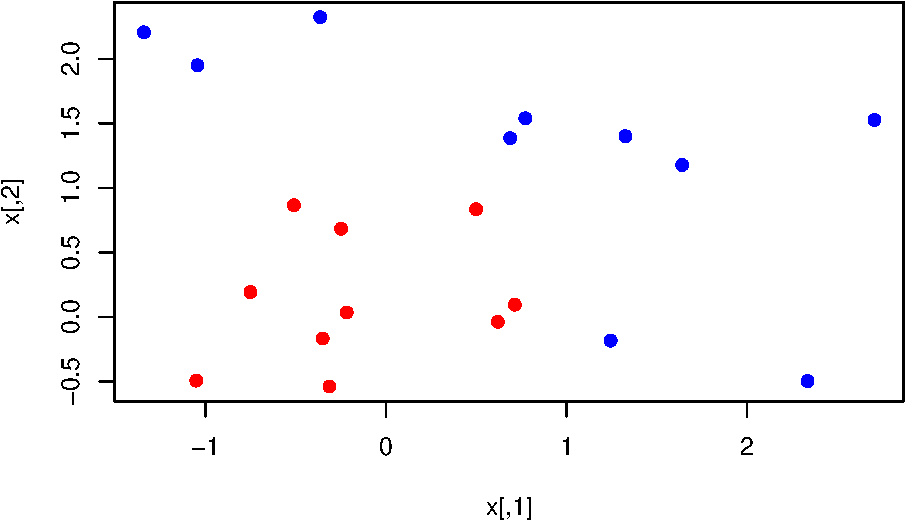
\includegraphics{3LinRegBEAMER_files/figure-beamer/unnamed-chunk-28-1.pdf}
\normalsize

\end{frame}

\begin{frame}

\textbf{A}: Ok linear assumption, but not constant spread.

\end{frame}

\begin{frame}[fragile]

\begin{block}{Normal Q-Q}

This plot shows if the residuals are Gaussian (normally) distributed. If
they follow a straigt line it is an indication that they are, and else
they are probably not.

\footnotesize

\begin{Shaded}
\begin{Highlighting}[]
\KeywordTok{ggplot}\NormalTok{(fit, }\KeywordTok{aes}\NormalTok{(}\DataTypeTok{sample =}\NormalTok{ .stdresid)) }\OperatorTok{+}\StringTok{ }\KeywordTok{stat_qq}\NormalTok{(}\DataTypeTok{pch =} \DecValTok{19}\NormalTok{) }\OperatorTok{+}\StringTok{ }\KeywordTok{geom_abline}\NormalTok{(}\DataTypeTok{intercept =} \DecValTok{0}\NormalTok{, }
    \DataTypeTok{slope =} \DecValTok{1}\NormalTok{, }\DataTypeTok{linetype =} \StringTok{"dotted"}\NormalTok{) }\OperatorTok{+}\StringTok{ }\KeywordTok{labs}\NormalTok{(}\DataTypeTok{x =} \StringTok{"Theoretical quantiles"}\NormalTok{, }
    \DataTypeTok{y =} \StringTok{"Standardized residuals"}\NormalTok{, }\DataTypeTok{title =} \StringTok{"Normal Q-Q"}\NormalTok{, }\DataTypeTok{subtitle =} \KeywordTok{deparse}\NormalTok{(fit}\OperatorTok{$}\NormalTok{call)) }\OperatorTok{+}\StringTok{ }
\StringTok{    }\KeywordTok{theme_minimal}\NormalTok{()}
\end{Highlighting}
\end{Shaded}

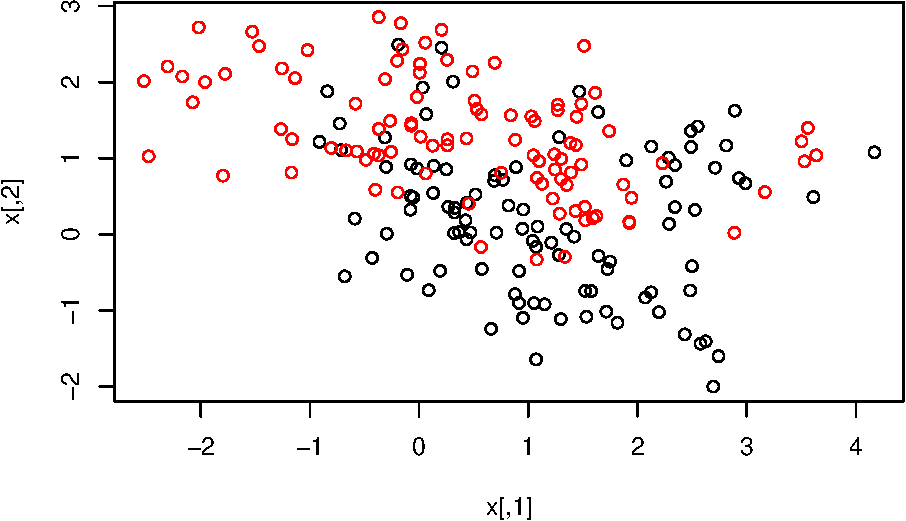
\includegraphics{3LinRegBEAMER_files/figure-beamer/unnamed-chunk-29-1.pdf}

\begin{Shaded}
\begin{Highlighting}[]
\KeywordTok{library}\NormalTok{(nortest)}
\KeywordTok{ad.test}\NormalTok{(}\KeywordTok{rstudent}\NormalTok{(fit))}
\end{Highlighting}
\end{Shaded}

\begin{verbatim}
## 
##  Anderson-Darling normality test
## 
## data:  rstudent(fit)
## A = 6.4123, p-value = 9.809e-16
\end{verbatim}

\normalsize

\end{block}

\end{frame}

\begin{frame}

\textbf{A}: Not normal.

\end{frame}

\begin{frame}

\begin{block}{Scale-location}

This is also called spread-location plot. It shows if the residuals are
spread equally along the ranges of predictors. Can be used to check the
assumption of equal variance (homoscedasticity). A good plot is one with
a horizontal line with randomly spread points.

Is this plot good for your data?

\end{block}

\end{frame}

\begin{frame}[fragile]

\footnotesize

\begin{Shaded}
\begin{Highlighting}[]
\KeywordTok{ggplot}\NormalTok{(fit, }\KeywordTok{aes}\NormalTok{(.fitted, }\KeywordTok{sqrt}\NormalTok{(}\KeywordTok{abs}\NormalTok{(.stdresid)))) }\OperatorTok{+}\StringTok{ }\KeywordTok{geom_point}\NormalTok{() }\OperatorTok{+}\StringTok{ }\KeywordTok{geom_smooth}\NormalTok{(}\DataTypeTok{se =} \OtherTok{FALSE}\NormalTok{, }
    \DataTypeTok{col =} \StringTok{"red"}\NormalTok{, }\DataTypeTok{size =} \FloatTok{0.5}\NormalTok{, }\DataTypeTok{method =} \StringTok{"loess"}\NormalTok{) }\OperatorTok{+}\StringTok{ }\KeywordTok{labs}\NormalTok{(}\DataTypeTok{x =} \StringTok{"Fitted values"}\NormalTok{, }
    \DataTypeTok{y =} \KeywordTok{expression}\NormalTok{(}\KeywordTok{sqrt}\NormalTok{(}\StringTok{"Standardized residuals"}\NormalTok{)), }\DataTypeTok{title =} \StringTok{"Scale-location"}\NormalTok{, }
    \DataTypeTok{subtitle =} \KeywordTok{deparse}\NormalTok{(fit}\OperatorTok{$}\NormalTok{call)) }\OperatorTok{+}\StringTok{ }\KeywordTok{theme_minimal}\NormalTok{()}
\end{Highlighting}
\end{Shaded}

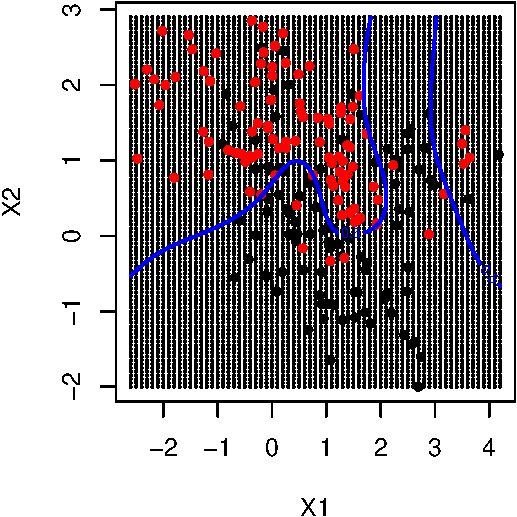
\includegraphics{3LinRegBEAMER_files/figure-beamer/unnamed-chunk-30-1.pdf}
\normalsize

\end{frame}

\begin{frame}

\textbf{A}: Confirms our observation of not constant variance.

\end{frame}

\begin{frame}[fragile]

\begin{block}{Residual vs Leverage}

This plot can reveal influential outliers. Not all outliers are
influential in linear regression; even though data have extreme values,
they might not be influential to determine the regression line (the
results don't differ much if they are removed from the data set). These
influential outliers can be seen as observations that does not get along
with the trend in the majority of the observations. In \texttt{plot.lm},
dashed lines are used to indicate the Cook's distance, instead of using
the size of the dots as is done here.

\end{block}

\end{frame}

\begin{frame}

Cook's distance is the Euclidean distance between the
\(\mathbf{\hat{y}}\) (the fitted values) and \(\mathbf{\hat{y}}_{(i)}\)
(the fitted values calculated when the \(i\)-th observation is omitted
from the regression). This is then a measure on how much the model is
influences by observation \(i\). The distance is scaled, and a rule of
thumb is to examine observations with Cook's distance larger than 1, and
give some attention to those with Cook's distance above 0.5.

Leverage is defined as the diagonal elements of the hat matrix, i.e.,
the leverage of the \(i\)-th data point is \(h_{ii}\) on the diagonal of
\(\mathbf{H = X(X^TX)^{-1}X^T}\). A large leverage indicated that the
observation (\(i\)) has a large influence on the estimation results, and
that the covariate values (\(\mathbf{x}_i\)) are unusual.

\end{frame}

\begin{frame}[fragile]

\footnotesize

\begin{Shaded}
\begin{Highlighting}[]
\KeywordTok{ggplot}\NormalTok{(fit, }\KeywordTok{aes}\NormalTok{(.hat, .stdresid)) }\OperatorTok{+}\StringTok{ }\KeywordTok{geom_smooth}\NormalTok{(}\DataTypeTok{se =} \OtherTok{FALSE}\NormalTok{, }\DataTypeTok{col =} \StringTok{"red"}\NormalTok{, }
    \DataTypeTok{size =} \FloatTok{0.5}\NormalTok{, }\DataTypeTok{method =} \StringTok{"loess"}\NormalTok{) }\OperatorTok{+}\StringTok{ }\KeywordTok{geom_point}\NormalTok{(}\KeywordTok{aes}\NormalTok{(}\DataTypeTok{size =}\NormalTok{ .cooksd)) }\OperatorTok{+}\StringTok{ }
\StringTok{    }\KeywordTok{scale_size_continuous}\NormalTok{(}\StringTok{"Cook's dist."}\NormalTok{) }\OperatorTok{+}\StringTok{ }\KeywordTok{labs}\NormalTok{(}\DataTypeTok{x =} \StringTok{"Leverage"}\NormalTok{, }\DataTypeTok{y =} \StringTok{"Standardized residuals"}\NormalTok{, }
    \DataTypeTok{title =} \StringTok{"Residuals vs Leverage"}\NormalTok{, }\DataTypeTok{subtitle =} \KeywordTok{deparse}\NormalTok{(fit}\OperatorTok{$}\NormalTok{call)) }\OperatorTok{+}\StringTok{ }
\StringTok{    }\KeywordTok{theme_minimal}\NormalTok{()}
\end{Highlighting}
\end{Shaded}

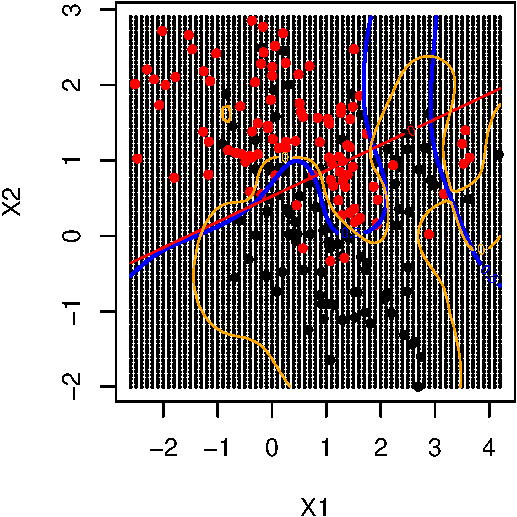
\includegraphics{3LinRegBEAMER_files/figure-beamer/unnamed-chunk-31-1.pdf}
\normalsize

\end{frame}

\begin{frame}

\textbf{A}:Some observations does not fit our model, but if we fit a
more complex model this may change.

\end{frame}

\begin{frame}[fragile]{Extensions and challenges in multiple regression}

The section is a self study section, where the dummy variable part is
the most important and will be used in this course.

\begin{block}{Qualitative covariates}

See
\href{https://www.youtube.com/watch?v=3T6RXmIHbJ4\&index=4\&list=PL5-da3qGB5IBSSCPANhTgrw82ws7w_or9}{Rob
Tibshirani explains - from ca 9 minutes}

Qualitative predictors can be included in a linear regression model by
introducing dummy variables

\textbf{Example}: consider our \texttt{rent} dataset with \texttt{rent}
as reponse, and continuous covariate \texttt{area} and categorical
covariate \texttt{location}. Let the \texttt{location} be a factor with
levels \texttt{average,\ good,\ top}.

\footnotesize

\begin{Shaded}
\begin{Highlighting}[]
\KeywordTok{library}\NormalTok{(gamlss.data)}
\KeywordTok{library}\NormalTok{(dplyr)}
\KeywordTok{library}\NormalTok{(GGally)}

\NormalTok{ds =}\StringTok{ }\NormalTok{dplyr}\OperatorTok{::}\KeywordTok{select}\NormalTok{(rent99, location, area, rent)}
\KeywordTok{levels}\NormalTok{(ds}\OperatorTok{$}\NormalTok{location)}
\CommentTok{# change to meaningful names}
\KeywordTok{levels}\NormalTok{(ds}\OperatorTok{$}\NormalTok{location) =}\StringTok{ }\KeywordTok{c}\NormalTok{(}\StringTok{"average"}\NormalTok{, }\StringTok{"good"}\NormalTok{, }\StringTok{"top"}\NormalTok{)}
\KeywordTok{ggpairs}\NormalTok{(ds)}
\end{Highlighting}
\end{Shaded}

\includegraphics{3LinRegBEAMER_files/figure-beamer/unnamed-chunk-32-1.pdf}
\normalsize

\textbf{Q}: comment on what you see in the \texttt{ggpairs} plot.

\end{block}

\end{frame}

\begin{frame}

Categorical covariates may either be ordered or unordered. We will only
consider unordered categories here. In general, we could like to
estimate regression coefficients for all levels for the categorical
covariates. However, if we want to include an intercept in our model we
can only include codings for one less variable than the number of levels
we have - or else our design matrix will not have full rank.

\textbf{Q}: Assume you have a categorical variable with three levels.
Check for yourself that making a design matrix with one intercept and
three columns with dummy (0-1) variable coding will result in a matrix
that is singular.

\end{frame}

\begin{frame}[fragile]

\footnotesize

\begin{Shaded}
\begin{Highlighting}[]
\CommentTok{# make 'wrong' dummy variable coding with 3 columns}
\NormalTok{n =}\StringTok{ }\KeywordTok{length}\NormalTok{(ds}\OperatorTok{$}\NormalTok{location)}
\NormalTok{X =}\StringTok{ }\KeywordTok{cbind}\NormalTok{(}\KeywordTok{rep}\NormalTok{(}\DecValTok{1}\NormalTok{, n), ds}\OperatorTok{$}\NormalTok{area, }\KeywordTok{rep}\NormalTok{(}\DecValTok{0}\NormalTok{, n), }\KeywordTok{rep}\NormalTok{(}\DecValTok{0}\NormalTok{, n), }\KeywordTok{rep}\NormalTok{(}\DecValTok{0}\NormalTok{, n))}
\NormalTok{X[ds}\OperatorTok{$}\NormalTok{location }\OperatorTok{==}\StringTok{ "average"}\NormalTok{, }\DecValTok{3}\NormalTok{] =}\StringTok{ }\DecValTok{1}
\NormalTok{X[ds}\OperatorTok{$}\NormalTok{location }\OperatorTok{==}\StringTok{ "good"}\NormalTok{, }\DecValTok{4}\NormalTok{] =}\StringTok{ }\DecValTok{1}
\NormalTok{X[ds}\OperatorTok{$}\NormalTok{location }\OperatorTok{==}\StringTok{ "top"}\NormalTok{, }\DecValTok{5}\NormalTok{] =}\StringTok{ }\DecValTok{1}
\NormalTok{X[}\KeywordTok{c}\NormalTok{(}\DecValTok{1}\NormalTok{, }\DecValTok{3}\NormalTok{, }\DecValTok{69}\NormalTok{), ]}
\end{Highlighting}
\end{Shaded}

\begin{verbatim}
##      [,1] [,2] [,3] [,4] [,5]
## [1,]    1   26    0    1    0
## [2,]    1   30    1    0    0
## [3,]    1   55    0    0    1
\end{verbatim}

\begin{Shaded}
\begin{Highlighting}[]
\KeywordTok{require}\NormalTok{(Matrix)}
\KeywordTok{dim}\NormalTok{(X)}
\end{Highlighting}
\end{Shaded}

\begin{verbatim}
## [1] 3082    5
\end{verbatim}

\begin{Shaded}
\begin{Highlighting}[]
\KeywordTok{rankMatrix}\NormalTok{(X)}
\end{Highlighting}
\end{Shaded}

\begin{verbatim}
## [1] 4
## attr(,"method")
## [1] "tolNorm2"
## attr(,"useGrad")
## [1] FALSE
## attr(,"tol")
## [1] 6.843415e-13
\end{verbatim}

\normalsize

\end{frame}

\begin{frame}

This is why we need to instead work with different ways of coding
categorical variables. One solution is to not include an intercept in
the model, but that is often not what we want. We will look at two other
solutions - one where we decide on a reference category (that we not
include in the coding, and therefore is kind of included in the
intercept - this is called ``treatment coding'') and one where we
require that the the sum of the coeffisients are zero (called ``effect
coding''). This mainly effects how we interpret parameter estimates and
communicate our findings to the world. We will here restrict our
discussion to ``treatment coding''.

\end{frame}

\begin{frame}[fragile]

If we fit a regression model with \texttt{lm} to the data with
\texttt{rent} as response and \texttt{area} and \texttt{location} as
covariates, a model matrix is made - and how to handle the categorical
variable is either specified the call to \texttt{lm} in
\texttt{contrasts=list(location="contr.treatment")} (or to model.matrix)
or globally for all categorical variables with
\texttt{options(contrasts=c("contr.treatment","contr.poly"))}- where
first element give choice for unordered factor (then treatment contrast
is default) and second for ordered (and then this polynomial contrast is
default). We will only work with unordered factors now.

\end{frame}

\begin{frame}

\begin{block}{Dummy variable coding}

This is the default coding. The reference level is automatically chosen
as the ``lowest'' level (sorted alphabetically). For our example this
means that the reference category for location is ``average''.

\[x_{i \text{locationgood}} = \begin{cases} 1 \text{ if } i \text{ -th location}=\text{"good"} \\ 0 \text{ if } i \text{ -th location }\neq\text{ "good"} \end{cases}\]
\[x_{i \text{locationtop}} = \begin{cases} 1 \text{ if } i \text{ -th location}=\text{"top"} \\ 0 \text{ if } i \text{ -th location }\neq\text{ "top"} \end{cases}\]
\[\begin{aligned} y_i &= \beta_0 + \beta_1 x_{i \text{area}} + \beta_2 x_{i \text{locationgood}}+\beta_3 x_{i \text{locationtop}} + \varepsilon_i\\\\ &= \begin{cases} \beta_0 + \beta_1 x_{i \text{area}}+ \beta_2 + \varepsilon_i  &\text{ if } i \text{ -th location}=\text{"good"}  \\ \beta_0 + \beta_1 x_{i \text{area}}+ \beta_3 + \varepsilon_i &\text{ if } i \text{ -th location}=\text{"top"} \\ \beta_0 + \varepsilon_i &\text{ if } i \text{ -th location}=\text{"average"}\end{cases}\end{aligned}\]

If we instead wanted ``good'' to be reference category we could relevel
the factor.

\end{block}

\end{frame}

\begin{frame}[fragile]

\begin{Shaded}
\begin{Highlighting}[]
\NormalTok{X1 =}\StringTok{ }\KeywordTok{model.matrix}\NormalTok{(}\OperatorTok{~}\NormalTok{area }\OperatorTok{+}\StringTok{ }\NormalTok{location, }\DataTypeTok{data =}\NormalTok{ ds)}
\NormalTok{X1[}\KeywordTok{c}\NormalTok{(}\DecValTok{1}\NormalTok{, }\DecValTok{3}\NormalTok{, }\DecValTok{69}\NormalTok{), ]}
\end{Highlighting}
\end{Shaded}

\begin{verbatim}
##    (Intercept) area locationgood locationtop
## 1            1   26            1           0
## 3            1   30            0           0
## 69           1   55            0           1
\end{verbatim}

\begin{Shaded}
\begin{Highlighting}[]
\NormalTok{ds}\OperatorTok{$}\NormalTok{locationRELEVEL =}\StringTok{ }\KeywordTok{relevel}\NormalTok{(ds}\OperatorTok{$}\NormalTok{location, }\DataTypeTok{ref =} \StringTok{"good"}\NormalTok{)}
\NormalTok{X2 =}\StringTok{ }\KeywordTok{model.matrix}\NormalTok{(}\OperatorTok{~}\NormalTok{area }\OperatorTok{+}\StringTok{ }\NormalTok{locationRELEVEL, }\DataTypeTok{data =}\NormalTok{ ds)}
\NormalTok{X2[}\KeywordTok{c}\NormalTok{(}\DecValTok{1}\NormalTok{, }\DecValTok{3}\NormalTok{, }\DecValTok{69}\NormalTok{), ]}
\end{Highlighting}
\end{Shaded}

\begin{verbatim}
##    (Intercept) area locationRELEVELaverage locationRELEVELtop
## 1            1   26                      0                  0
## 3            1   30                      1                  0
## 69           1   55                      0                  1
\end{verbatim}

So, what does this mean in practice? Model 1 has \texttt{average} as
reference category and model 2 \texttt{good}.

\end{frame}

\begin{frame}[fragile]

\begin{Shaded}
\begin{Highlighting}[]
\NormalTok{fit1 =}\StringTok{ }\KeywordTok{lm}\NormalTok{(rent }\OperatorTok{~}\StringTok{ }\NormalTok{area }\OperatorTok{+}\StringTok{ }\NormalTok{location, }\DataTypeTok{data =}\NormalTok{ ds, }\DataTypeTok{contrasts =} \KeywordTok{list}\NormalTok{(}\DataTypeTok{location =} \StringTok{"contr.treatment"}\NormalTok{))}
\KeywordTok{summary}\NormalTok{(fit1)}
\end{Highlighting}
\end{Shaded}

\begin{verbatim}
## 
## Call:
## lm(formula = rent ~ area + location, data = ds, contrasts = list(location = "contr.treatment"))
## 
## Residuals:
##     Min      1Q  Median      3Q     Max 
## -790.98 -100.89   -4.87   94.47 1004.98 
## 
## Coefficients:
##              Estimate Std. Error t value Pr(>|t|)    
## (Intercept)  128.0867     8.6947  14.732  < 2e-16 ***
## area           4.7056     0.1202  39.142  < 2e-16 ***
## locationgood  28.0040     5.8662   4.774 1.89e-06 ***
## locationtop  131.1075    18.2614   7.180 8.73e-13 ***
## ---
## Signif. codes:  0 '***' 0.001 '**' 0.01 '*' 0.05 '.' 0.1 ' ' 1
## 
## Residual standard error: 157.1 on 3078 degrees of freedom
## Multiple R-squared:  0.3555, Adjusted R-squared:  0.3549 
## F-statistic:   566 on 3 and 3078 DF,  p-value: < 2.2e-16
\end{verbatim}

\begin{Shaded}
\begin{Highlighting}[]
\NormalTok{fit2 =}\StringTok{ }\KeywordTok{lm}\NormalTok{(rent }\OperatorTok{~}\StringTok{ }\NormalTok{area }\OperatorTok{+}\StringTok{ }\NormalTok{locationRELEVEL, }\DataTypeTok{data =}\NormalTok{ ds, }\DataTypeTok{contrasts =} \KeywordTok{list}\NormalTok{(}\DataTypeTok{locationRELEVEL =} \StringTok{"contr.treatment"}\NormalTok{))}
\KeywordTok{summary}\NormalTok{(fit2)}
\end{Highlighting}
\end{Shaded}

\begin{verbatim}
## 
## Call:
## lm(formula = rent ~ area + locationRELEVEL, data = ds, contrasts = list(locationRELEVEL = "contr.treatment"))
## 
## Residuals:
##     Min      1Q  Median      3Q     Max 
## -790.98 -100.89   -4.87   94.47 1004.98 
## 
## Coefficients:
##                        Estimate Std. Error t value Pr(>|t|)    
## (Intercept)            156.0907     9.4950  16.439  < 2e-16 ***
## area                     4.7056     0.1202  39.142  < 2e-16 ***
## locationRELEVELaverage -28.0040     5.8662  -4.774 1.89e-06 ***
## locationRELEVELtop     103.1034    18.4021   5.603 2.30e-08 ***
## ---
## Signif. codes:  0 '***' 0.001 '**' 0.01 '*' 0.05 '.' 0.1 ' ' 1
## 
## Residual standard error: 157.1 on 3078 degrees of freedom
## Multiple R-squared:  0.3555, Adjusted R-squared:  0.3549 
## F-statistic:   566 on 3 and 3078 DF,  p-value: < 2.2e-16
\end{verbatim}

\textbf{Q}: Comment on the print-out. How do we interpret the intercept
estimate?

\end{frame}

\begin{frame}[fragile]

\begin{block}{Interactions}

See
\href{https://www.youtube.com/watch?v=IFzVxLv0TKQ\&list=PL5-da3qGB5IBSSCPANhTgrw82ws7w_or9\&index=5}{Trevor
Hastie explains}

To illustrate how interactions between covariates can be included we use
the \texttt{ozone} data set from the \texttt{ElemStatLearn} library.
This data set is measurements from 1973 in New York and contains 111
observations of the following variables:

\begin{itemize}
\tightlist
\item
  \texttt{ozone} : ozone concentration (ppm)
\item
  \texttt{radiation} : solar radiation (langleys)
\item
  \texttt{temperature} : daily maximum temperature (F)
\item
  \texttt{wind} : wind speed (mph)
\end{itemize}

We start by fitting a multiple linear regression model to the data, with
\texttt{ozone} as our response variable and \texttt{temperature} and
\texttt{wind} as covariates.

\begin{verbatim}
##   ozone radiation temperature wind
## 1    41       190          67  7.4
## 2    36       118          72  8.0
## 3    12       149          74 12.6
## 4    18       313          62 11.5
## 5    23       299          65  8.6
## 6    19        99          59 13.8
\end{verbatim}

\end{block}

\end{frame}

\begin{frame}[fragile]

\small

\begin{verbatim}
## 
## Call:
## lm(formula = ozone ~ temperature + wind, data = ozone)
## 
## Residuals:
##     Min      1Q  Median      3Q     Max 
## -42.160 -13.209  -3.089  10.588  98.470 
## 
## Coefficients:
##             Estimate Std. Error t value Pr(>|t|)    
## (Intercept) -67.2008    23.6083  -2.846  0.00529 ** 
## temperature   1.8265     0.2504   7.293 5.32e-11 ***
## wind         -3.2993     0.6706  -4.920 3.12e-06 ***
## ---
## Signif. codes:  0 '***' 0.001 '**' 0.01 '*' 0.05 '.' 0.1 ' ' 1
## 
## Residual standard error: 21.72 on 108 degrees of freedom
## Multiple R-squared:  0.5817, Adjusted R-squared:  0.574 
## F-statistic:  75.1 on 2 and 108 DF,  p-value: < 2.2e-16
\end{verbatim}

\normalsize

\end{frame}

\begin{frame}[fragile]

The model can be written as:
\[Y = \beta_0 + \beta_1 x_t + \beta_2 x_w + \varepsilon\] In this model
we have assumed that increasing the value of one covariate is
independent of the other covariates. For example: by increasing the
\texttt{temperature} by one-unit always increases the response value by
\(\beta_2 \approx 1.651\), regardless of the value of \texttt{wind}.

\end{frame}

\begin{frame}[fragile]

However, one might think that the covariate \texttt{wind} (wind speed)
might act differently upon \texttt{ozone} for different values of
\texttt{temperature} and vice verse.
\[\begin{aligned} Y &= \beta_0 +  \beta_1 x_t + \beta_2 x_w + \beta_3\cdot(x_t  \cdot x_w) +\varepsilon \\ &= \beta_0 +  (\beta_1 + \beta_3 x_w) \cdot x_t + \beta_2 x_w + \varepsilon \\ &= \beta_0 + \beta_1 x_t + (\beta_2 + \beta_3 x_t) \cdot x_w + \varepsilon \end{aligned}.\]
We fit this model in \texttt{R}. An interaction term can be included in
the model using the \texttt{*} symbol.

\textbf{Q:} Look at the \texttt{summary} below. Is this a better model
than without the interaction term? It the term significant?

\end{frame}

\begin{frame}[fragile]

\footnotesize

\begin{Shaded}
\begin{Highlighting}[]
\NormalTok{ozone.int =}\StringTok{ }\KeywordTok{lm}\NormalTok{(ozone }\OperatorTok{~}\StringTok{ }\NormalTok{temperature }\OperatorTok{+}\StringTok{ }\NormalTok{wind }\OperatorTok{+}\StringTok{ }\NormalTok{temperature }\OperatorTok{*}\StringTok{ }\NormalTok{wind, }\DataTypeTok{data =}\NormalTok{ ozone)}
\KeywordTok{summary}\NormalTok{(ozone.int)}
\end{Highlighting}
\end{Shaded}

\begin{verbatim}
## 
## Call:
## lm(formula = ozone ~ temperature + wind + temperature * wind, 
##     data = ozone)
## 
## Residuals:
##     Min      1Q  Median      3Q     Max 
## -40.929 -11.190  -3.037   8.209  97.440 
## 
## Coefficients:
##                    Estimate Std. Error t value Pr(>|t|)    
## (Intercept)      -239.94146   48.59004  -4.938 2.92e-06 ***
## temperature         4.00151    0.59311   6.747 8.02e-10 ***
## wind               13.60882    4.28070   3.179  0.00193 ** 
## temperature:wind   -0.21747    0.05446  -3.993  0.00012 ***
## ---
## Signif. codes:  0 '***' 0.001 '**' 0.01 '*' 0.05 '.' 0.1 ' ' 1
## 
## Residual standard error: 20.36 on 107 degrees of freedom
## Multiple R-squared:  0.636,  Adjusted R-squared:  0.6258 
## F-statistic: 62.31 on 3 and 107 DF,  p-value: < 2.2e-16
\end{verbatim}

\normalsize

\end{frame}

\begin{frame}

Below we see that the interaction term is highly significant. The
\(p\)-value is very small, so that there is strong evidence that
\(\beta_3 \neq 0\). Furthermore, \(R^2_{\text{adj}}\) has increased,
indicating that more of the variability in the data has been explained
by the model (than without the interaction).

\end{frame}

\begin{frame}[fragile]

\emph{Interpretation of the interaction term:}

\begin{itemize}
\item
  If we now increase the \texttt{temperature} by \(10^{\circ}\) F, the
  increase in \texttt{wind} speed will be
  \[(\hat \beta_1+\hat \beta_3 \cdot x_w) \cdot 10 = (4.0 -0.22 \cdot x_w) \cdot 10 = 40-2.2 x_w \text{ units}.\]
\item
  If we increase the \texttt{wind} speed by 10 mph, the increase in
  \texttt{temperature} will be
  \[(\hat \beta_2 + \hat \beta_3 \cdot x_t) \cdot 10 = (14 -0.22 \cdot x_t) \cdot 10 = 140-2.2 x_t \text{ units}.\]
\end{itemize}

\end{frame}

\begin{frame}[fragile]

\textbf{The hierarchical principle}

It is possible that the interaction term is higly significant, but the
main effects are not.

In our \texttt{ozone.int} model above: the main effects are
\texttt{temperature} and \texttt{wind}. The hierarchical principle
states that if we include an interaction term in our model, the main
effects are also to be included, even if they are not significant. This
means that if the coefficients \(\hat \beta_1\) or \(\hat \beta_2\)
would be insignificant, while the coefficient \(\hat \beta_3\) is
significant, \(\hat \beta_1\) and \(\hat \beta_2\) should still be
included in the model.

There reasons for this is that a model with interaction terms, but
without the main effects is hard to interpret.

\end{frame}

\begin{frame}[fragile]

\begin{block}{Interactions between qualitative (discrete) and
quantitative (continuous) covariates}

We create a new variable \texttt{temp.cat} which is a
\texttt{temperature} as a qualitative covariate with two levels and fit
the model:
\[\begin{aligned}y&=\beta_0 + \beta_1 x_w + \begin{cases} \beta_2 + \beta_3  x_w  &\text{ if temperature="low"}\\ 0 &\text{ if temperature = "high"}\end{cases} \\\\ &= \begin{cases} (\beta_0 + \beta_2) + (\beta_1 + \beta_3) \cdot x_w &\text{ if temperature="low"}\\ \beta_0 + \beta_1 x_w &\text{ if temperature="high""} \end{cases} \end{aligned}\]

\end{block}

\end{frame}

\begin{frame}[fragile]

\footnotesize

\begin{Shaded}
\begin{Highlighting}[]
\NormalTok{temp.cat =}\StringTok{ }\KeywordTok{ifelse}\NormalTok{(ozone}\OperatorTok{$}\NormalTok{temperature }\OperatorTok{<}\StringTok{ }\KeywordTok{mean}\NormalTok{(ozone}\OperatorTok{$}\NormalTok{temperature), }\StringTok{"low"}\NormalTok{, }
    \StringTok{"high"}\NormalTok{)}
\NormalTok{ozone2 =}\StringTok{ }\KeywordTok{cbind}\NormalTok{(ozone, temp.cat)}
\KeywordTok{print}\NormalTok{(}\KeywordTok{head}\NormalTok{(ozone2))}
\end{Highlighting}
\end{Shaded}

\begin{verbatim}
##   ozone radiation temperature wind temp.cat
## 1    41       190          67  7.4      low
## 2    36       118          72  8.0      low
## 3    12       149          74 12.6      low
## 4    18       313          62 11.5      low
## 5    23       299          65  8.6      low
## 6    19        99          59 13.8      low
\end{verbatim}

\begin{Shaded}
\begin{Highlighting}[]
\NormalTok{ozone.int2 =}\StringTok{ }\KeywordTok{lm}\NormalTok{(ozone }\OperatorTok{~}\StringTok{ }\NormalTok{wind }\OperatorTok{+}\StringTok{ }\NormalTok{temp.cat }\OperatorTok{+}\StringTok{ }\NormalTok{temp.cat }\OperatorTok{*}\StringTok{ }\NormalTok{wind, }\DataTypeTok{data =}\NormalTok{ ozone2)}
\KeywordTok{summary}\NormalTok{(ozone.int2)}
\end{Highlighting}
\end{Shaded}

\begin{verbatim}
## 
## Call:
## lm(formula = ozone ~ wind + temp.cat + temp.cat * wind, data = ozone2)
## 
## Residuals:
##     Min      1Q  Median      3Q     Max 
## -53.291  -9.091  -1.307  11.227  71.815 
## 
## Coefficients:
##                  Estimate Std. Error t value Pr(>|t|)    
## (Intercept)      119.0450     7.5004  15.872  < 2e-16 ***
## wind              -6.7235     0.8195  -8.204 5.61e-13 ***
## temp.catlow      -92.6316    12.9466  -7.155 1.09e-10 ***
## wind:temp.catlow   6.0544     1.1999   5.046 1.86e-06 ***
## ---
## Signif. codes:  0 '***' 0.001 '**' 0.01 '*' 0.05 '.' 0.1 ' ' 1
## 
## Residual standard error: 20.26 on 107 degrees of freedom
## Multiple R-squared:  0.6393, Adjusted R-squared:  0.6291 
## F-statistic:  63.2 on 3 and 107 DF,  p-value: < 2.2e-16
\end{verbatim}

\normalsize

\end{frame}

\begin{frame}[fragile]

\footnotesize

\begin{Shaded}
\begin{Highlighting}[]
\NormalTok{interceptlow =}\StringTok{ }\KeywordTok{coef}\NormalTok{(ozone.int2)[}\DecValTok{1}\NormalTok{] }\OperatorTok{+}\StringTok{ }\KeywordTok{coef}\NormalTok{(ozone.int2)[}\DecValTok{3}\NormalTok{]}
\NormalTok{slopelow =}\StringTok{ }\KeywordTok{coef}\NormalTok{(ozone.int2)[}\DecValTok{2}\NormalTok{] }\OperatorTok{+}\StringTok{ }\KeywordTok{coef}\NormalTok{(ozone.int2)[}\DecValTok{4}\NormalTok{]}
\NormalTok{intercepthigh =}\StringTok{ }\KeywordTok{coef}\NormalTok{(ozone.int2)[}\DecValTok{1}\NormalTok{]}
\NormalTok{slopehigh =}\StringTok{ }\KeywordTok{coef}\NormalTok{(ozone.int2)[}\DecValTok{2}\NormalTok{]}
\KeywordTok{ggplot}\NormalTok{(ozone) }\OperatorTok{+}\StringTok{ }\KeywordTok{geom_line}\NormalTok{(}\KeywordTok{aes}\NormalTok{(}\DataTypeTok{y =}\NormalTok{ interceptlow }\OperatorTok{+}\StringTok{ }\NormalTok{slopelow }\OperatorTok{*}\StringTok{ }\NormalTok{wind, }\DataTypeTok{x =}\NormalTok{ wind), }
    \DataTypeTok{col =} \StringTok{"blue"}\NormalTok{) }\OperatorTok{+}\StringTok{ }\KeywordTok{geom_line}\NormalTok{(}\KeywordTok{aes}\NormalTok{(}\DataTypeTok{y =}\NormalTok{ intercepthigh }\OperatorTok{+}\StringTok{ }\NormalTok{slopehigh }\OperatorTok{*}\StringTok{ }\NormalTok{wind, }
    \DataTypeTok{x =}\NormalTok{ wind), }\DataTypeTok{col =} \StringTok{"red"}\NormalTok{) }\OperatorTok{+}\StringTok{ }\KeywordTok{ylab}\NormalTok{(}\StringTok{"ozone"}\NormalTok{) }\OperatorTok{+}\StringTok{ }\KeywordTok{theme_minimal}\NormalTok{()}
\end{Highlighting}
\end{Shaded}

\includegraphics{3LinRegBEAMER_files/figure-beamer/unnamed-chunk-40-1.pdf}

\normalsize

\end{frame}

\begin{frame}

\begin{block}{Nonlinearity}

We may extend the linear model to handle non-linear relationships by
using polynomial regression - as we did in Module 2 in our bias-variance
trade-off example.

More on non-linearity in Module 7.

\end{block}

\end{frame}

\begin{frame}

\begin{block}{Optional: Projection matrices}

First, we define predictions as \(\hat{\bf Y}={\bf X}\hat{\beta}\), and
inserted the ML (and LS) estimate we get
\(\hat{\bf Y}={\bf X}({\bf X}^T{\bf X})^{-1}{\bf X}^T{\bf Y}\).

We define the projection matrix
\[  {\bf H}={\bf X}({\bf X}^T{\bf X})^{-1} {\bf X}^T\] called the
\emph{hat matrix}. This simplifies the notation for the predictions,
\[\hat{\bf Y}={\bf H}{\bf Y}\] so the hat matrix is putting the hat on
the response \({\bf Y}\).

In addition we define residuals as

\begin{align*}
{\bf e}&={\bf Y}-\hat{\bf Y} \\
{\bf e}&={\bf Y}-{\bf HY}=({\bf I-H}){\bf Y}\\
\end{align*}

so we have a second projection matrix
\[ {\bf I-H}={\bf I}-{\bf X}({\bf X}^T{\bf X})^{-1} {\bf X}^T \]

\end{block}

\end{frame}

\begin{frame}

\begin{block}{Optional: Geometry of Least Squares (involving our two
projection matrices)}

\begin{itemize}
\tightlist
\item
  Mean response vector: \(\text{E}({\bf Y})={\bf X}{\boldsymbol \beta}\)
\item
  As \(\beta\) varies, \({\bf X}\beta\) spans the model plane of all
  linear combinations. I.e. the space spanned by the columns of
  \({\bf X}\): the column-space of \({\bf X}\).
\item
  Due to random error (and unobserved covariates), \({\bf Y}\) is not
  exactly a linear combination of the columns of \({\bf X}\).
\item
  LS-estimation chooses \(\hat{\beta}\) such that \({\bf X}\hat{\beta}\)
  is the point in the column-space of \({\bf X}\) that is closes to
  \({\bf Y}\).
\item
  The residual vector
  \(\hat{\varepsilon}={\bf Y}-\hat{{\bf Y}}=({\bf I-H}){\bf Y}\) is
  perpendicular to the column-space of \({\bf X}\).
\item
  Multiplication by \({\bf H}={\bf X}({\bf X}^T{\bf X})^{-1}{\bf X}^T\)
  projects a vector onto the column-space of \({\bf X}\).
\item
  Multiplication by
  \({\bf I-H}={\bf I}-{\bf X}({\bf X}^T{\bf X})^{-1}{\bf X}^T\) projects
  a vector onto the space perpendicular to the column-space of
  \({\bf X}\).
\end{itemize}

\end{block}

\end{frame}

\begin{frame}

\end{frame}

\begin{frame}{Important results in multiple linear regression}

\begin{itemize}
\tightlist
\item
  Linear regression assumes a linear relationship between the response
  variable and the covariates.
\item
  Simple linear regression has only one covariate and has the form
  \(Y = \beta_0 + \beta_1 X + \varepsilon\).
\item
  Muliple linear regression has \(p\) covariates and has the form
  \(Y = \beta_0 + \beta_1 X_1 + \beta_2 X_2 + ... + \beta_p X_p + \varepsilon\).
\item
  Quantitative (categorical) covariates can be included using dummy
  variables.
\item
  Correlations among the covariates can mask each others effects in the
  linear model.
\item
  Parameter estimates can be obtained by minimizing the least squares
  (RSS) or by maximum likelihood estimation.
\item
  We can calculate the standard errors of the parameter estimates, and
  use this to obtain confidence intervals.
\item
  We can test the hypothesis of \(H_0 : \beta_j = 0\) against
  \(H_1: \beta_j \neq 0\) by a t-test.
\item
  We use the \(F\)-statistic to test if at least one of the covariates
  are useful.
\end{itemize}

\end{frame}

\begin{frame}

\begin{itemize}
\item
  Not only additive effects: Interactions between covariates can be
  included in the model (also between qualitative and quantitative
  covariates).
\item
  Transformations of the response variable or of a covariate can be
  useful if the relationship is not linear. A linear model can then be
  fit to the transformed variables.
\item
  The overall accuracy of the model can be evaluated by calculating the
  \(R^2\) statistic, AIC score and by using diagnostic plots.
\item
  Model selection can not be based on RSS or \(R^2\).
\item
  Multiple linear regression might require subset selection if the
  number of covariates is high.
\end{itemize}

\end{frame}

\begin{frame}[fragile]{Recommended exercises}

\begin{block}{Problem 1: Compulsory exercise in 2018}

There will be a very similar regression problem in the compulsory
exercise 1 in 2019!

The Framingham Heart Study is a study of the etiology (i.e.~underlying
causes) of cardiovascular disease, with participants from the community
of Framingham in Massachusetts, USA. For more more information about the
Framingham Heart Study visit
\url{https://www.framinghamheartstudy.org/}. The dataset used in here is
subset of a teaching version of the Framingham data, used with
permission from the Framingham Heart Study.

We will focus on modelling systolic blood pressure using data from n =
2600 persons. For each person in the data set we have measurements of
the seven variables

\begin{itemize}
\tightlist
\item
  \texttt{SYSBP} systolic blood pressure,
\item
  \texttt{SEX} 1=male, 2=female,
\item
  \texttt{AGE} age in years at examination,
\item
  \texttt{CURSMOKE} current cigarette smoking at examination: 0=not
  current smoker, 1= current smoker,
\item
  \texttt{BMI} body mass index,
\item
  \texttt{TOTCHOL} serum total cholesterol, and
\item
  \texttt{BPMEDS} use of anti-hypertensive medication at examination:
  0=not currently using, 1=currently using.
\end{itemize}

A multiple normal linear regression model was fitted to the data set
with \texttt{-1/sqrt(SYSBP)} as response and all the other variables as
covariates.

\begin{Shaded}
\begin{Highlighting}[]
\KeywordTok{library}\NormalTok{(ggplot2)}
\NormalTok{data =}\StringTok{ }\KeywordTok{read.table}\NormalTok{(}\StringTok{"https://www.math.ntnu.no/emner/TMA4268/2018v/data/SYSBPreg3uid.txt"}\NormalTok{)}
\KeywordTok{dim}\NormalTok{(data)}
\KeywordTok{colnames}\NormalTok{(data)}
\NormalTok{modelA =}\StringTok{ }\KeywordTok{lm}\NormalTok{(}\OperatorTok{-}\DecValTok{1}\OperatorTok{/}\KeywordTok{sqrt}\NormalTok{(SYSBP) }\OperatorTok{~}\StringTok{ }\NormalTok{., }\DataTypeTok{data =}\NormalTok{ data)}
\KeywordTok{summary}\NormalTok{(modelA)}
\end{Highlighting}
\end{Shaded}

\end{block}

\begin{block}{a) Understanding model output}

We name the model fitted above \texttt{modelA}.

\begin{itemize}
\tightlist
\item
  Write down the equation for the fitted \texttt{modelA}.
\item
  Explain (with words and formula) what the following in the
  \texttt{summary}-output means.
\item
  \texttt{Estimate} - in particular interpretation of \texttt{Intercept}
\item
  \texttt{Std.Error}
\item
  \texttt{t\ value}
\item
  \texttt{Pr(\textgreater{}\textbar{}t\textbar{})}
\item
  \texttt{Residual\ standard\ error}
\item
  \texttt{F-statistic}
\end{itemize}

\end{block}

\begin{block}{b) Model fit}

\begin{itemize}
\tightlist
\item
  What is the proportion of variability explained by the fitted
  \texttt{modelA}? Comment.
\item
  Use diagnostic plots of ``fitted values vs.~standardized residuals''"
  and ``QQ-plot of standardized residuals'' (see code below) to assess
  the model fit.
\item
  Now fit a model, call this \texttt{modelB}, with \texttt{SYSBP} as
  response, and the same covariates as for \texttt{modelA}. Would you
  prefer to use \texttt{modelA} or \texttt{modelB} when the aim is to
  make inference about the systolic blood pressure?
\end{itemize}

\begin{Shaded}
\begin{Highlighting}[]
\CommentTok{# residuls vs fitted}
\KeywordTok{ggplot}\NormalTok{(modelA, }\KeywordTok{aes}\NormalTok{(.fitted, .resid)) }\OperatorTok{+}\StringTok{ }\KeywordTok{geom_point}\NormalTok{(}\DataTypeTok{pch =} \DecValTok{21}\NormalTok{) }\OperatorTok{+}\StringTok{ }\KeywordTok{geom_hline}\NormalTok{(}\DataTypeTok{yintercept =} \DecValTok{0}\NormalTok{, }
    \DataTypeTok{linetype =} \StringTok{"dashed"}\NormalTok{) }\OperatorTok{+}\StringTok{ }\KeywordTok{geom_smooth}\NormalTok{(}\DataTypeTok{se =} \OtherTok{FALSE}\NormalTok{, }\DataTypeTok{col =} \StringTok{"red"}\NormalTok{, }\DataTypeTok{size =} \FloatTok{0.5}\NormalTok{, }
    \DataTypeTok{method =} \StringTok{"loess"}\NormalTok{) }\OperatorTok{+}\StringTok{ }\KeywordTok{labs}\NormalTok{(}\DataTypeTok{x =} \StringTok{"Fitted values"}\NormalTok{, }\DataTypeTok{y =} \StringTok{"Residuals"}\NormalTok{, }\DataTypeTok{title =} \StringTok{"Fitted values vs. residuals"}\NormalTok{, }
    \DataTypeTok{subtitle =} \KeywordTok{deparse}\NormalTok{(modelA}\OperatorTok{$}\NormalTok{call))}

\CommentTok{# qq-plot of residuals}
\KeywordTok{ggplot}\NormalTok{(modelA, }\KeywordTok{aes}\NormalTok{(}\DataTypeTok{sample =}\NormalTok{ .stdresid)) }\OperatorTok{+}\StringTok{ }\KeywordTok{stat_qq}\NormalTok{(}\DataTypeTok{pch =} \DecValTok{19}\NormalTok{) }\OperatorTok{+}\StringTok{ }\KeywordTok{geom_abline}\NormalTok{(}\DataTypeTok{intercept =} \DecValTok{0}\NormalTok{, }
    \DataTypeTok{slope =} \DecValTok{1}\NormalTok{, }\DataTypeTok{linetype =} \StringTok{"dotted"}\NormalTok{) }\OperatorTok{+}\StringTok{ }\KeywordTok{labs}\NormalTok{(}\DataTypeTok{x =} \StringTok{"Theoretical quantiles"}\NormalTok{, }
    \DataTypeTok{y =} \StringTok{"Standardized residuals"}\NormalTok{, }\DataTypeTok{title =} \StringTok{"Normal Q-Q"}\NormalTok{, }\DataTypeTok{subtitle =} \KeywordTok{deparse}\NormalTok{(modelA}\OperatorTok{$}\NormalTok{call))}

\CommentTok{# normality test}
\KeywordTok{library}\NormalTok{(nortest)}
\KeywordTok{ad.test}\NormalTok{(}\KeywordTok{rstudent}\NormalTok{(modelA))}
\end{Highlighting}
\end{Shaded}

\end{block}

\begin{block}{c) Confidence interval and hypothesis test}

We use \texttt{modelA} and focus on addressing the association between
BMI and the response.

\begin{itemize}
\tightlist
\item
  What is the estimate \(\hat{\beta}_{\text{BMI}}\) (numerically)?
\item
  Explain how to interpret the estimated coefficient
  \(\hat{\beta}_{\text{BMI}}\).
\item
  Construct a 99\% confidence interval for \(\beta_{\text{BMI}}\) (write
  out the formula and calculate the interval numerically). Explain what
  this interval tells you.
\item
  From this confidence interval, is it possible for you know anything
  about the value of the \(p\)-value for the test
  \(H_0: \beta_{\text{BMI}}=0\) vs. \(H_1:\beta_{\text{BMI}} \neq 0\)?
  Explain.
\end{itemize}

\end{block}

\begin{block}{d) Prediction}

Consider a 56 year old man who is smoking. He is 1.75 meters tall and
his weight is 89 kilograms. His serum total cholesterol is 200 mg/dl and
he is not using anti-hypertensive medication.

\begin{Shaded}
\begin{Highlighting}[]
\KeywordTok{names}\NormalTok{(data)}
\NormalTok{new =}\StringTok{ }\KeywordTok{data.frame}\NormalTok{(}\DataTypeTok{SEX =} \DecValTok{1}\NormalTok{, }\DataTypeTok{AGE =} \DecValTok{56}\NormalTok{, }\DataTypeTok{CURSMOKE =} \DecValTok{1}\NormalTok{, }\DataTypeTok{BMI =} \DecValTok{89}\OperatorTok{/}\FloatTok{1.75}\OperatorTok{^}\DecValTok{2}\NormalTok{, }\DataTypeTok{TOTCHOL =} \DecValTok{200}\NormalTok{, }
    \DataTypeTok{BPMEDS =} \DecValTok{0}\NormalTok{)}
\end{Highlighting}
\end{Shaded}

\begin{itemize}
\tightlist
\item
  What is your best guess for his \texttt{-1/sqrt(SYSBP)}? To get a best
  guess for his \texttt{SYSBP} you may take the inverse function of
  \texttt{-1/sqrt}.
\end{itemize}

(Comment: Is that allowed - to only do the inverse? Yes, that could be
the result of a first order Taylor expansion approximation. If you think
this is interesting you can read more from page 36 here:
\url{https://www.math.ntnu.no/emner/TMA4267/2017v/L12.pdf} - but that is
not on the reading list of this course. You have probably used this
result in your physics courses.)

\begin{itemize}
\tightlist
\item
  Construct a 90\% prediction interval for his systolic blood pressure
  \texttt{SYSBP}. Comment. Hint: first contruct values on the scale of
  the response \texttt{-1/sqrt(SYSBP)} and then transform the upper and
  lower limits of the prediction interval.
\item
  Do you find this prediction interval useful? Comment.
\end{itemize}

\end{block}

\end{frame}

\begin{frame}

\begin{block}{Problem 2: Theoretical questions}

\begin{block}{a)}

A core finding is \(\hat{\boldsymbol\beta}\).
\[ \hat{\boldsymbol\beta}=({\bf X}^T{\bf X})^{-1} {\bf X}^T {\bf Y}\]
with
\(\hat{\boldsymbol\beta}\sim N_{p}(\boldsymbol\beta,\sigma^2({\bf X}^T{\bf X})^{-1})\).

\begin{itemize}
\tightlist
\item
  Show that \(\hat{\boldsymbol\beta}\) has this distribution with the
  given mean and covariance matrix.
\item
  What do you need to assume to get to this result?
\item
  What does this imply for the distribution of the \(j\)th element of
  \(\hat{\beta}\)?
\item
  In particular, how can we calculate the variance of \(\hat{\beta}_j\)?
\end{itemize}

\end{block}

\begin{block}{b)}

What is the interpretation of a 95\% confidence interval? Hint: repeat
experiment (on \(Y\)), on average how many CIs cover the true
\(\beta_j\)?

\end{block}

\begin{block}{c)}

What is the interpretation of a 95\% prediction interval? Hint: repeat
experiment (on \(Y\)) for a given \({\bf x}_0\).

\end{block}

\begin{block}{d)}

Construct a 95\% CI for \({\bf x}_0^T \beta\). Explain what is the
connections between a CI for \(\beta_j\), a CI for \({\bf x}_0^T \beta\)
and a PI for \(Y\) at \({\bf x}_0\).

\end{block}

\begin{block}{e)}

Explain the difference between \emph{error} and \emph{residual}. What
are the properties of the raw residuals? Why don't we want to use the
raw residuals for model check? What is our solution to this?

\end{block}

\begin{block}{f)}

Consider a multiple linear regression model \(A\) and a submodel \(B\)
(all parameters in \(B\) are in \(A\) also). We say that \(B\) is nested
within \(A\). Assume that regression parameters are estimated using
least squares. Why is then the following true: RSS for model \(A\) will
always be smaller or equal to RSS for model \(B\). And thus, \(R^2\) for
model \(A\) can never be worse than \(R^2\) for model B. (See also
Problem 3d below.)

\end{block}

\end{block}

\end{frame}

\begin{frame}[fragile]

\begin{block}{Problem 3: Munich Rent index}

\begin{block}{a)}

Fit the regression model with first \texttt{rent} and then
\texttt{rentsqm} as reponse and following covariates: \texttt{area},
\texttt{location} (dummy variable coding using location2 and location3,
just write \texttt{as.factor(location)}), \texttt{bath},
\texttt{kitchen} and \texttt{cheating} (central heating).

Look at diagnostic plots for the two fits. Which response do you prefer?

Consentrate on the response-model you choose for the rest of the tasks.

\end{block}

\begin{block}{b)}

Explain what the parameter estimates mean in practice. In particular,
what is the interpretation of the intercept?

\end{block}

\begin{block}{c)}

Go through the summary printout and explain all parts.

\end{block}

\begin{block}{d)}

Now we add random noise as a covariance, but simulating the IQ of the
landlord of each appartment. Observe that \(R^2\) increases (or stays
unchanged) and RSS decreases (or stays the same) if we add IQ as
covariate, but \(R^2_{\text{adj}}\) decreases. What does this tell you
about model selection and overfitting?

For the code - what is the connection between \texttt{sigma} and RSS?

\begin{Shaded}
\begin{Highlighting}[]
\NormalTok{orgfit =}\StringTok{ }\KeywordTok{lm}\NormalTok{(rent }\OperatorTok{~}\StringTok{ }\NormalTok{area }\OperatorTok{+}\StringTok{ }\KeywordTok{as.factor}\NormalTok{(location) }\OperatorTok{+}\StringTok{ }\NormalTok{bath }\OperatorTok{+}\StringTok{ }\NormalTok{kitchen }\OperatorTok{+}\StringTok{ }\NormalTok{cheating, }
    \DataTypeTok{data =}\NormalTok{ rent99)}
\KeywordTok{summary}\NormalTok{(orgfit)}
\KeywordTok{set.seed}\NormalTok{(}\DecValTok{1}\NormalTok{)  }\CommentTok{#to be able to reproduce results}
\NormalTok{n =}\StringTok{ }\KeywordTok{dim}\NormalTok{(rent99)[}\DecValTok{1}\NormalTok{]}
\NormalTok{IQ =}\StringTok{ }\KeywordTok{rnorm}\NormalTok{(n, }\DecValTok{100}\NormalTok{, }\DecValTok{16}\NormalTok{)}
\NormalTok{fitIQ =}\StringTok{ }\KeywordTok{lm}\NormalTok{(rent }\OperatorTok{~}\StringTok{ }\NormalTok{area }\OperatorTok{+}\StringTok{ }\KeywordTok{as.factor}\NormalTok{(location) }\OperatorTok{+}\StringTok{ }\NormalTok{bath }\OperatorTok{+}\StringTok{ }\NormalTok{kitchen }\OperatorTok{+}\StringTok{ }\NormalTok{cheating }\OperatorTok{+}\StringTok{ }
\StringTok{    }\NormalTok{IQ, }\DataTypeTok{data =}\NormalTok{ rent99)}
\KeywordTok{summary}\NormalTok{(fitIQ)}

\KeywordTok{summary}\NormalTok{(orgfit)}\OperatorTok{$}\NormalTok{sigma}
\KeywordTok{summary}\NormalTok{(fitIQ)}\OperatorTok{$}\NormalTok{sigma}

\KeywordTok{summary}\NormalTok{(orgfit)}\OperatorTok{$}\NormalTok{r.squared}
\KeywordTok{summary}\NormalTok{(fitIQ)}\OperatorTok{$}\NormalTok{r.squared}
\KeywordTok{summary}\NormalTok{(orgfit)}\OperatorTok{$}\NormalTok{adj.r.squared}
\KeywordTok{summary}\NormalTok{(fitIQ)}\OperatorTok{$}\NormalTok{adj.r.squared}
\end{Highlighting}
\end{Shaded}

\begin{verbatim}
## 
## Call:
## lm(formula = rent ~ area + as.factor(location) + bath + kitchen + 
##     cheating, data = rent99)
## 
## Residuals:
##     Min      1Q  Median      3Q     Max 
## -633.41  -89.17   -6.26   82.96 1000.76 
## 
## Coefficients:
##                      Estimate Std. Error t value Pr(>|t|)    
## (Intercept)          -21.9733    11.6549  -1.885   0.0595 .  
## area                   4.5788     0.1143  40.055  < 2e-16 ***
## as.factor(location)2  39.2602     5.4471   7.208 7.14e-13 ***
## as.factor(location)3 126.0575    16.8747   7.470 1.04e-13 ***
## bath1                 74.0538    11.2087   6.607 4.61e-11 ***
## kitchen1             120.4349    13.0192   9.251  < 2e-16 ***
## cheating1            161.4138     8.6632  18.632  < 2e-16 ***
## ---
## Signif. codes:  0 '***' 0.001 '**' 0.01 '*' 0.05 '.' 0.1 ' ' 1
## 
## Residual standard error: 145.2 on 3075 degrees of freedom
## Multiple R-squared:  0.4504, Adjusted R-squared:  0.4494 
## F-statistic:   420 on 6 and 3075 DF,  p-value: < 2.2e-16
## 
## 
## Call:
## lm(formula = rent ~ area + as.factor(location) + bath + kitchen + 
##     cheating + IQ, data = rent99)
## 
## Residuals:
##     Min      1Q  Median      3Q     Max 
## -630.95  -89.50   -6.12   82.62  995.76 
## 
## Coefficients:
##                      Estimate Std. Error t value Pr(>|t|)    
## (Intercept)          -41.3879    19.5957  -2.112   0.0348 *  
## area                   4.5785     0.1143  40.056  < 2e-16 ***
## as.factor(location)2  39.2830     5.4467   7.212 6.90e-13 ***
## as.factor(location)3 126.3356    16.8748   7.487 9.18e-14 ***
## bath1                 74.1979    11.2084   6.620 4.23e-11 ***
## kitchen1             120.0756    13.0214   9.221  < 2e-16 ***
## cheating1            161.4450     8.6625  18.637  < 2e-16 ***
## IQ                     0.1940     0.1574   1.232   0.2179    
## ---
## Signif. codes:  0 '***' 0.001 '**' 0.01 '*' 0.05 '.' 0.1 ' ' 1
## 
## Residual standard error: 145.2 on 3074 degrees of freedom
## Multiple R-squared:  0.4507, Adjusted R-squared:  0.4494 
## F-statistic: 360.3 on 7 and 3074 DF,  p-value: < 2.2e-16
## 
## [1] 145.1879
## [1] 145.1757
## [1] 0.4504273
## [1] 0.4506987
## [1] 0.449355
## [1] 0.4494479
\end{verbatim}

\end{block}

\begin{block}{e)}

We now want to use model selection to arrive at a good model. Start by
defining which covariates you want to include and how to code them (use
dummy variable coding of \texttt{location}). What about year of
construction - is that a linear covariate? Maybe you want to make
intervals in time instead? Linear or categorical for the time? What
about the \texttt{district}? We leave that since we have not talked
about how to use spatial covariates.

Hint: if you want to test out interval versions of year of construction
the function \texttt{mutate} (from \texttt{dplyr}) is useful:

\begin{Shaded}
\begin{Highlighting}[]
\NormalTok{rent99 <-}\StringTok{ }\NormalTok{rent99 }\OperatorTok\StringTok{ }\KeywordTok{mutate}\NormalTok{(}\DataTypeTok{yearc.cat =} \KeywordTok{cut}\NormalTok{(yearc, }\DataTypeTok{breaks =} \KeywordTok{c}\NormalTok{(}\OperatorTok{-}\OtherTok{Inf}\NormalTok{, }\KeywordTok{seq}\NormalTok{(}\DecValTok{1920}\NormalTok{, }
    \DecValTok{2000}\NormalTok{, }\DecValTok{10}\NormalTok{)), }\DataTypeTok{labels =} \DecValTok{10} \OperatorTok{*}\StringTok{ }\DecValTok{1}\OperatorTok{:}\DecValTok{9}\NormalTok{))}
\end{Highlighting}
\end{Shaded}

More on \texttt{dplyr}: Tutorial:
\url{http://genomicsclass.github.io/book/pages/dplyr_tutorial.html} and
Cheat sheet (data wrangling):
\url{https://www.rstudio.com/wp-content/uploads/2015/02/data-wrangling-cheatsheet.pdf}
and dplyr in particular:
\url{https://github.com/rstudio/cheatsheets/raw/master/source/pdfs/data-transformation-cheatsheet.pdf}

\end{block}

\begin{block}{f)}

(More on this in Module 6.)

There are many ways to perform model selection for multiple linear
regression. One possibility is best subsets, which can be done using the
\texttt{regsubsets} function from library \texttt{leaps}. Assume your
``full'' model fitted by \texttt{lm} is called \texttt{fit}. You may
define \texttt{x} from \texttt{model.matrix(fit){[},-1{]}} (not
including the intercept term), and then run
\texttt{best=regsubsets(x=model.matrix(fit){[},-1{]},y=rent99\$rent)}
and look at \texttt{summary(best)}. Explain the print-out (with all the
stars). Using the Mallows Cp (named \texttt{cp} in the list from
\texttt{summary(best)}) will give the same result at using AIC (which is
not available in this function). What is your preferred model? Hint:
look at the R-code in Problem 2 (Figure 3) from the TMA4267V2017 exam:
\href{https://www.math.ntnu.no/emner/TMA4267/2017v/Exam/eV2017Enew.pdf}{pdf},
and maybe the solutions for the interpretation
\href{https://www.math.ntnu.no/emner/TMA4267/2017v/Exam/mergedLFV2017.pdf}{pdf}

\end{block}

\end{block}

\end{frame}

\begin{frame}[fragile]

\begin{block}{Problem 4: Simulations in R}

\begin{block}{a}

Make R code that shows the interpretation of a 95\% CI for \(\beta_j\).
Hint: Theoretical question a.

\end{block}

\begin{block}{b}

Make R code that shows the interpretation of a 95\% PI for a new
response at \({\bf x}_0\). Hint: Theoretical question b.

\end{block}

\begin{block}{c.}

For simple linear regression, simulate at data set with homoscedastic
errors and with heteroscedastic errors. Here is a suggestion of one
solution - not using \texttt{ggplot}. You use \texttt{ggplot}. Why this?
To see how things looks when the model is correct and wrong.

\begin{Shaded}
\begin{Highlighting}[]
\CommentTok{# Homoscedastic errore}
\NormalTok{n =}\StringTok{ }\DecValTok{1000}
\NormalTok{x =}\StringTok{ }\KeywordTok{seq}\NormalTok{(}\OperatorTok{-}\DecValTok{3}\NormalTok{, }\DecValTok{3}\NormalTok{, }\DataTypeTok{length =}\NormalTok{ n)}
\NormalTok{beta0 =}\StringTok{ }\OperatorTok{-}\DecValTok{1}
\NormalTok{beta1 =}\StringTok{ }\DecValTok{2}
\NormalTok{xbeta =}\StringTok{ }\NormalTok{beta0 }\OperatorTok{+}\StringTok{ }\NormalTok{beta1 }\OperatorTok{*}\StringTok{ }\NormalTok{x}
\NormalTok{sigma =}\StringTok{ }\DecValTok{1}
\NormalTok{e1 =}\StringTok{ }\KeywordTok{rnorm}\NormalTok{(n, }\DataTypeTok{mean =} \DecValTok{0}\NormalTok{, }\DataTypeTok{sd =}\NormalTok{ sigma)}
\NormalTok{y1 =}\StringTok{ }\NormalTok{xbeta }\OperatorTok{+}\StringTok{ }\NormalTok{e1}
\NormalTok{ehat1 =}\StringTok{ }\KeywordTok{residuals}\NormalTok{(}\KeywordTok{lm}\NormalTok{(y1 }\OperatorTok{~}\StringTok{ }\NormalTok{x))}
\KeywordTok{plot}\NormalTok{(x, y1, }\DataTypeTok{pch =} \DecValTok{20}\NormalTok{)}
\KeywordTok{abline}\NormalTok{(beta0, beta1, }\DataTypeTok{col =} \DecValTok{1}\NormalTok{)}
\KeywordTok{plot}\NormalTok{(x, e1, }\DataTypeTok{pch =} \DecValTok{20}\NormalTok{)}
\KeywordTok{abline}\NormalTok{(}\DataTypeTok{h =} \DecValTok{0}\NormalTok{, }\DataTypeTok{col =} \DecValTok{2}\NormalTok{)}
\CommentTok{# Heteroscedastic errors}
\NormalTok{sigma =}\StringTok{ }\NormalTok{(}\FloatTok{0.1} \OperatorTok{+}\StringTok{ }\FloatTok{0.3} \OperatorTok{*}\StringTok{ }\NormalTok{(x }\OperatorTok{+}\StringTok{ }\DecValTok{3}\NormalTok{))}\OperatorTok{^}\DecValTok{2}
\NormalTok{e2 =}\StringTok{ }\KeywordTok{rnorm}\NormalTok{(n, }\DecValTok{0}\NormalTok{, }\DataTypeTok{sd =}\NormalTok{ sigma)}
\NormalTok{y2 =}\StringTok{ }\NormalTok{xbeta }\OperatorTok{+}\StringTok{ }\NormalTok{e2}
\NormalTok{ehat2 =}\StringTok{ }\KeywordTok{residuals}\NormalTok{(}\KeywordTok{lm}\NormalTok{(y2 }\OperatorTok{~}\StringTok{ }\NormalTok{x))}
\KeywordTok{plot}\NormalTok{(x, y2, }\DataTypeTok{pch =} \DecValTok{20}\NormalTok{)}
\KeywordTok{abline}\NormalTok{(beta0, beta1, }\DataTypeTok{col =} \DecValTok{2}\NormalTok{)}
\KeywordTok{plot}\NormalTok{(x, e2, }\DataTypeTok{pch =} \DecValTok{20}\NormalTok{)}
\KeywordTok{abline}\NormalTok{(}\DataTypeTok{h =} \DecValTok{0}\NormalTok{, }\DataTypeTok{col =} \DecValTok{2}\NormalTok{)}
\end{Highlighting}
\end{Shaded}

\end{block}

\begin{block}{d.}

All this fuss about raw, standardized and studentized residuals- does
really matter in practice? Below is one example where the raw residuals
are rather different from the standardized, but the standardized is
identical to the studentized. Can you come up with a simulation model
where the standardized and studentized are very different? Hint: what
about at smaller sample size?

\begin{Shaded}
\begin{Highlighting}[]
\NormalTok{n =}\StringTok{ }\DecValTok{1000}
\NormalTok{beta =}\StringTok{ }\KeywordTok{matrix}\NormalTok{(}\KeywordTok{c}\NormalTok{(}\DecValTok{0}\NormalTok{, }\DecValTok{1}\NormalTok{, }\DecValTok{1}\OperatorTok{/}\DecValTok{2}\NormalTok{, }\DecValTok{1}\OperatorTok{/}\DecValTok{3}\NormalTok{), }\DataTypeTok{ncol =} \DecValTok{1}\NormalTok{)}
\KeywordTok{set.seed}\NormalTok{(}\DecValTok{123}\NormalTok{)}
\NormalTok{x1 =}\StringTok{ }\KeywordTok{rnorm}\NormalTok{(n, }\DecValTok{0}\NormalTok{, }\DecValTok{1}\NormalTok{)}
\NormalTok{x2 =}\StringTok{ }\KeywordTok{rnorm}\NormalTok{(n, }\DecValTok{0}\NormalTok{, }\DecValTok{2}\NormalTok{)}
\NormalTok{x3 =}\StringTok{ }\KeywordTok{rnorm}\NormalTok{(n, }\DecValTok{0}\NormalTok{, }\DecValTok{3}\NormalTok{)}
\NormalTok{X =}\StringTok{ }\KeywordTok{cbind}\NormalTok{(}\KeywordTok{rep}\NormalTok{(}\DecValTok{1}\NormalTok{, n), x1, x2, x3)}
\NormalTok{y =}\StringTok{ }\NormalTok{X }\OperatorTok\StringTok{ }\NormalTok{beta }\OperatorTok{+}\StringTok{ }\KeywordTok{rnorm}\NormalTok{(n, }\DecValTok{0}\NormalTok{, }\DecValTok{2}\NormalTok{)}
\NormalTok{fit =}\StringTok{ }\KeywordTok{lm}\NormalTok{(y }\OperatorTok{~}\StringTok{ }\NormalTok{x1 }\OperatorTok{+}\StringTok{ }\NormalTok{x2 }\OperatorTok{+}\StringTok{ }\NormalTok{x3)}
\NormalTok{yhat =}\StringTok{ }\KeywordTok{predict}\NormalTok{(fit)}
\KeywordTok{summary}\NormalTok{(fit)}
\NormalTok{ehat =}\StringTok{ }\KeywordTok{residuals}\NormalTok{(fit)}
\NormalTok{estand =}\StringTok{ }\KeywordTok{rstandard}\NormalTok{(fit)}
\NormalTok{estud =}\StringTok{ }\KeywordTok{rstudent}\NormalTok{(fit)}
\KeywordTok{plot}\NormalTok{(yhat, ehat, }\DataTypeTok{pch =} \DecValTok{20}\NormalTok{)}
\KeywordTok{points}\NormalTok{(yhat, estand, }\DataTypeTok{pch =} \DecValTok{20}\NormalTok{, }\DataTypeTok{col =} \DecValTok{2}\NormalTok{)}
\end{Highlighting}
\end{Shaded}

\end{block}

\end{block}

\end{frame}

\begin{frame}{ Further reading }

\begin{itemize}
\tightlist
\item
  Need details on the simple linear regression: From TMA4240/TMA4245
  Statistics we have the thematic page for
  \href{https://wiki.math.ntnu.no/tma4245/tema/begreper/regression}{Simple
  linear regression (in Norwegian)}.
\item
  Need more advanced thory: Theoretical version (no simple linear
  regression) from TMA4315 Generalized linear models H2018:
  \href{https://www.math.ntnu.no/emner/TMA4315/2018h/2MLR.html}{TMA4315M2:
  Multiple linear regression}
\item
  Slightly different presentation (more focus on multivariate normal
  theory):
  \href{https://www.math.ntnu.no/emner/TMA4267/2017v/TMA4267V2017Part2.pdf}{Slides
  and written material from TMA4267}
\item
  And, same source, but now
  \href{http://www.math.ntnu.no/emner/TMA4267/2017v/TMA4267V2017Part3.pdf}{Slides
  and written material from TMA4267 Linear Statistical Models in 2017,
  Part 3: Hypothesis testing and ANOVA}
\item
  \href{https://www.youtube.com/playlist?list=PL5-da3qGB5IBSSCPANhTgrw82ws7w_or9}{Videoes
  on YouTube by the authors of ISL, Chapter 2}
\end{itemize}

\end{frame}

\begin{frame}[fragile]{ R packages}

If you want to look at the .Rmd file and \texttt{knit} it, you need to
first install the following packages (only once).

\begin{Shaded}
\begin{Highlighting}[]
\CommentTok{# packages to install before knitting this R Markdown file to knit}
\CommentTok{# the Rmd}
\KeywordTok{install.packages}\NormalTok{(}\StringTok{"knitr"}\NormalTok{)}
\KeywordTok{install.packages}\NormalTok{(}\StringTok{"rmarkdown"}\NormalTok{)}

\CommentTok{# nice tables in Rmd}
\KeywordTok{install.packages}\NormalTok{(}\StringTok{"kableExtra"}\NormalTok{)}

\CommentTok{# cool layout for the Rmd}
\KeywordTok{install.packages}\NormalTok{(}\StringTok{"prettydoc"}\NormalTok{)  }\CommentTok{# alternative to github}

\CommentTok{# plotting}
\KeywordTok{install.packages}\NormalTok{(}\StringTok{"ggplot2"}\NormalTok{)  }\CommentTok{# cool plotting}
\KeywordTok{install.packages}\NormalTok{(}\StringTok{"ggpubr"}\NormalTok{)  }\CommentTok{# for many ggplots}
\KeywordTok{install.packages}\NormalTok{(}\StringTok{"GGally"}\NormalTok{)  }\CommentTok{# for ggpairs}
\CommentTok{# datasets}
\KeywordTok{install.packages}\NormalTok{(}\StringTok{"ElemStatLearn"}\NormalTok{)  }\CommentTok{# for ozone data set}
\KeywordTok{install.packages}\NormalTok{(}\StringTok{"gamlss.data"}\NormalTok{)  }\CommentTok{#rent index data set here}
\CommentTok{# methods}
\KeywordTok{install.packages}\NormalTok{(}\StringTok{"nortest"}\NormalTok{)  }\CommentTok{#test for normality - e.g. Anderson-Darling}

\KeywordTok{install.packages}\NormalTok{(}\StringTok{"car"}\NormalTok{)  }\CommentTok{# vif}
\KeywordTok{library}\NormalTok{(Matrix)}
\KeywordTok{install.packages}\NormalTok{(}\StringTok{"reshape"}\NormalTok{)}
\KeywordTok{install.packages}\NormalTok{(}\StringTok{"corrplot"}\NormalTok{)}
\KeywordTok{install.packages}\NormalTok{(}\StringTok{"tidyverse"}\NormalTok{)}
\end{Highlighting}
\end{Shaded}

\end{frame}

\begin{frame}{Acknowledgements}

Thanks to Julia Debik for contributing to this module page.

\end{frame}

\end{document}
